% !TeX spellcheck = fr_FR
\documentclass[11pt,a5paper,twoside]{book}
%format A5
%\usepackage[top=25mm, bottom=20mm, outer=20mm, inner=25mm]{geometry}
%Format Royal
\usepackage[paperwidth=156mm, paperheight=234mm,top=25mm, bottom=20mm, outer=20mm, inner=25mm]{geometry}
\usepackage[utf8]{inputenc}
\usepackage{CJKutf8} 
%\usepackage{xeCJK} 
%\setCJKmainfont{AR PL UMing TW MBE}
\usepackage[T1]{fontenc}
\usepackage{makeidx}
\usepackage{graphicx}
\usepackage[hidelinks]{hyperref}
%Restricts floats within section
\usepackage{placeins}
%Subfigures
\usepackage{subfigure}
%Header and footer control
%\usepackage{fancyhdr}
%\pagestyle{fancy}
%Verbatim and multi-line comments
\usepackage{verbatim}
\usepackage[french]{babel}
%
%Caption control
\usepackage[font=small,format=plain,labelfont=bf,labelsep=endash,textfont=up]{caption}
\captionsetup{figurename=Fig.}
%Include des macros Pinyin pour traitement de-macro avant pandoc ou tex4ebook
\usepackage{Pinyin-private}
\usepackage[abs]{overpic}
\usepackage{color}
\usepackage{anyfontsize}
%Pour les unités physiques, kg, g, cm, etc.
\usepackage[squaren,Gray]{SIunits}
%==============================================================
\title{{\Huge \TAIJIJIAN{}\\}{\huge l'escrime du \Taiji{}}}
\author{{\Large Frédéric Plewniak}}
\makeindex
%\tolerance=600
\begin{document}
\newcommand{\fiche}[1]{}
\setcounter{secnumdepth}{0}
%\renewcommand{\chaptermark}[1]{ \markboth{#1}{} }
\renewcommand{\sectionmark}[1]{ \markright{#1}{} }
%Set the level of sections in table of contents
\setcounter{tocdepth}{1}
\frontmatter
\begin{titlepage}
%\setcounter{page}{0}
%\newgeometry{top=0mm, bottom=0mm, outer=0mm, inner=0mm, hoffset=-6mm,voffset=0mm}
%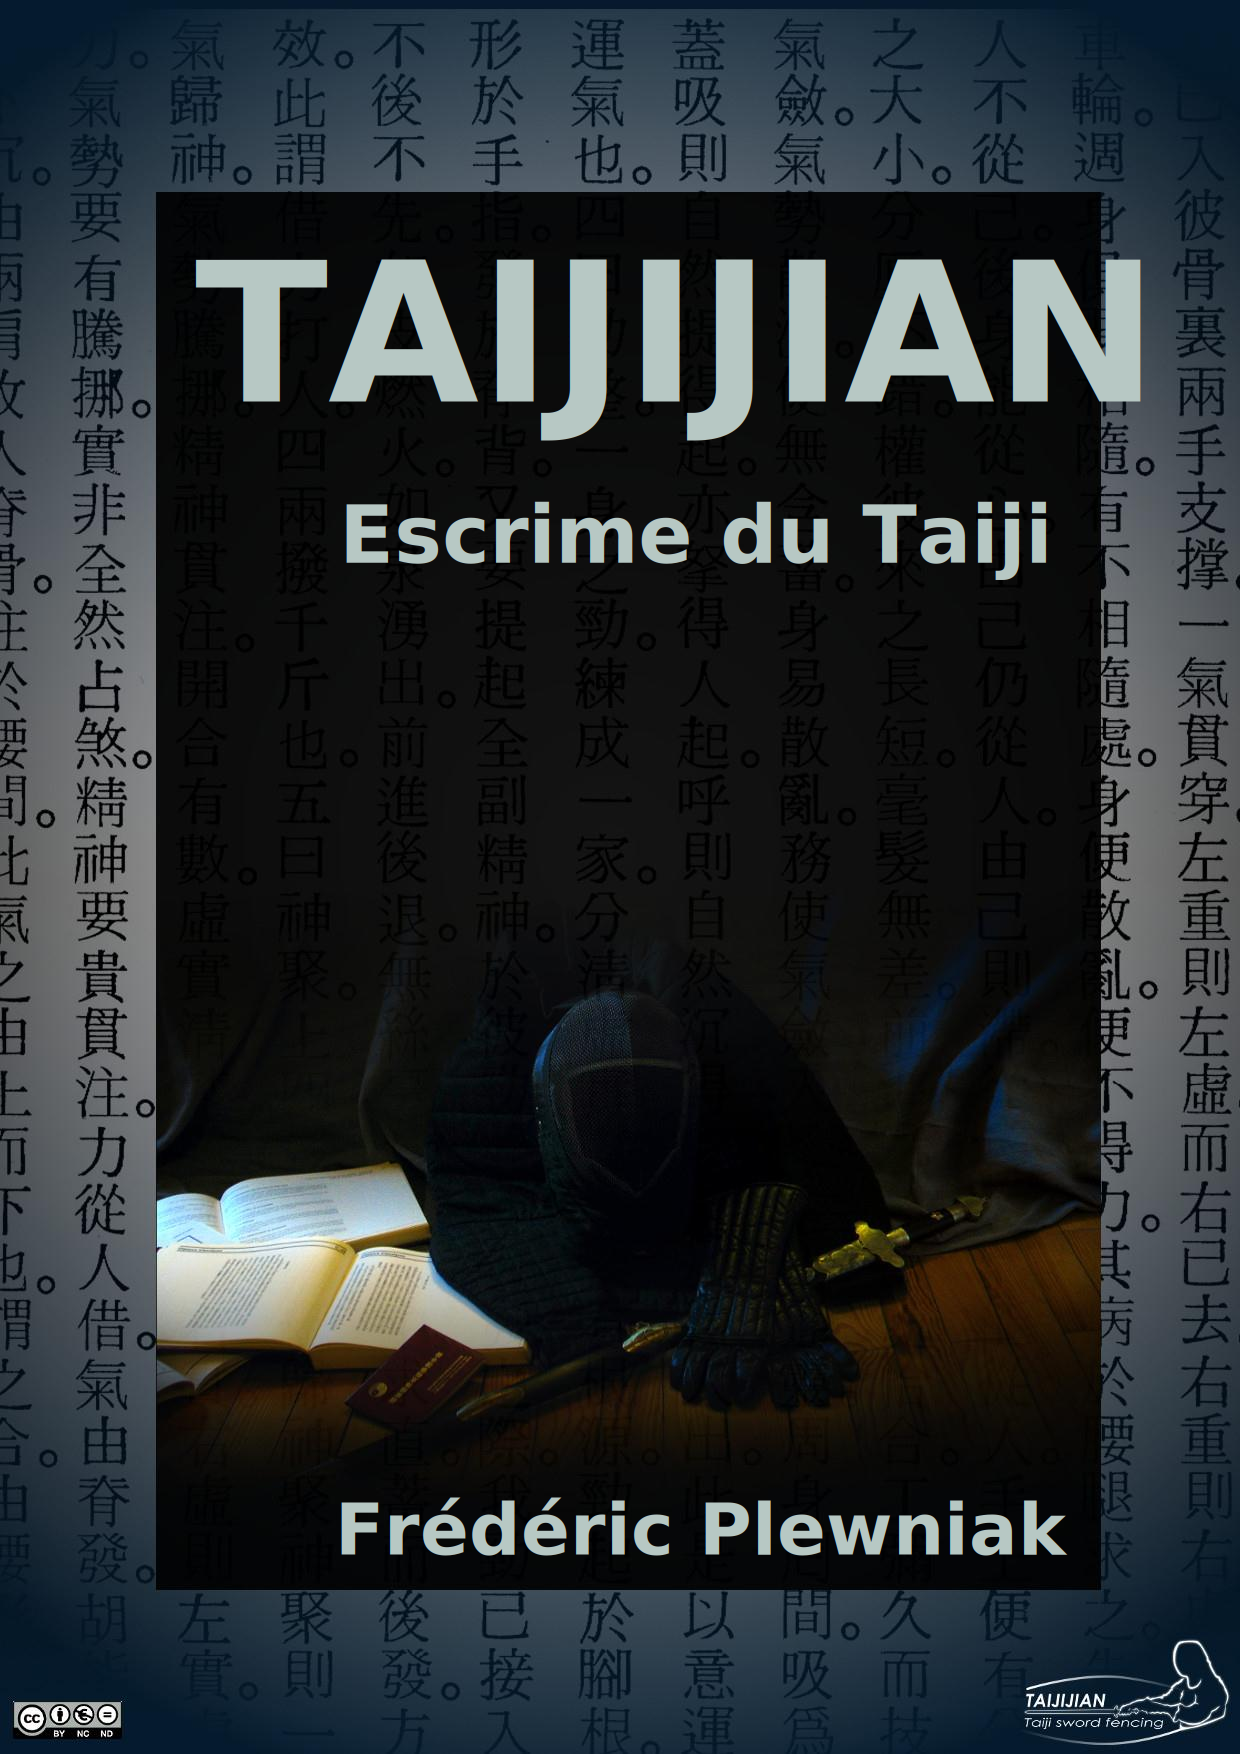
\includegraphics[width=\paperwidth]{../../Images/CouverturePDF_French}
\setlength\unitlength{1mm}
\newgeometry{top=0mm, bottom=0mm, outer=0mm, inner=0mm, hoffset=-6mm,voffset=1mm}
\begin{overpic}[width=\paperwidth]%
{../../Images/CouverturePDF_Royal}
\put(28,180){\color{white}{{\upshape\fontfamily{ppl}\fontseries{b}\fontsize{50}{60}\selectfont \TAIJIJIAN{}}}}
\put(30,165){\color{white}{{\upshape\fontfamily{ppl}\fontseries{m}\fontsize{35}{30}\selectfont Escrime du \Taiji{}}}}

\put(70,25){\color{white}{{\scshape\fontfamily{pbk}\fontseries{l}\fontsize{20}{20}\selectfont Frédéric Plewniak}}}
\end{overpic}
\thispagestyle{empty}
\end{titlepage}
\restoregeometry
\maketitle
\thispagestyle{empty}
\setcounter{page}{0}
% !TeX spellcheck = en_GB
\scriptsize
\par\vspace*{\fill}
\begin{center}

\includegraphics[height=2em]{../../Licence/by-nc-nd}

\copyright{} Fr\'{e}d\'{e}ric Plewniak 2014-\the\year
\end{center}

\begin{center}
This work is licensed under the Creative Commons Attribution-NonCommercial-NoDerivatives 4.0 International License. 

http://creativecommons.org/licenses/by-nc-nd/4.0/legalcode
\end{center}
\medskip
\subsubsection{{\footnotesize You are free to:}}
\paragraph{}\textbf{Share} \textendash{} copy and redistribute the material in any medium or format
\paragraph{}The licensor cannot revoke these freedoms as long as you follow the license terms.

\subsubsection{{\footnotesize Under the following terms:}}
\begin{itemize}
\item{\textbf{Attribution}  \textendash{} You must give appropriate credit, provide a link to the license, and indicate if changes were made. You may do so in any reasonable manner, but not in any way that suggests the licensor endorses you or your use.}

\item{\textbf{NonCommercial}  \textendash{} You may not use the material for commercial purposes.}

\item{\textbf{NoDerivatives}  \textendash{} If you remix, transform, or build upon the material, you may not distribute the modified material.}

\item{\textbf{No additional restrictions} — You may not apply legal terms or technological measures that legally restrict others from doing anything the license permits.}
\end{itemize}

\subsubsection{ {\footnotesize Notices:}}

\paragraph{}You do not have to comply with the license for elements of the material in the public domain or where your use is permitted by an applicable exception or limitation.
\paragraph{}No warranties are given. The license may not give you all of the permissions necessary for your intended use. For example, other rights such as publicity, privacy, or moral rights may limit how you use the material.
\clearpage
\normalsize
\tableofcontents
\listoffigures
% !TeX spellcheck = fr_FR
\chapter{Avant-propos}\label{avant-propos}

\paragraph*{}
Dans la plupart des styles et des écoles, le \Taijijian{} est presque exclusivement étudié sous la forme d'enchaînements, le plus souvent sans se soucier particulièrement de ses racines martiales.
Bien que l'on rencontre aujourd'hui un intérêt croissant pour des exercices avec partenaire, principalement d'épées collantes, les applications martiales sont très rarement présentées et lorsqu'elles le sont, se limitent souvent à des explications et justifications martiales des mouvements de la forme.
Ce qu'on pourrait vraiment appeler une escrime du \Taijijian{} est encore plus rarement évoqué ou pratiqué.

\paragraph*{}
Le présent travail est une tentative de jeter un pont entre la pratique des formes d'épée du \Taiji{} et une escrime du \Taijijian{}.
C'est le résultat de près de quinze ans de recherche et d'expérimentation, à la découverte de la dimension martiale du \Taijijian{}, depuis les notions élémentaires d'escrime, les applications martiales de la forme, jusqu'à la pratique d'assauts libres dans le respect des principes du {T\`{a}ij\'{\i}}. 
Les sources de ce travail sont ancrées dans la tradition du \Yangjia{} \Michuan{} \Taijijian{} transmise par Maître Wang Yen-nien, et en particulier la forme d'épée \Kunlun{}, connue aussi dans ce style sous le nom d'\emph{Épée ancienne}.
L'escrime historique européenne des XIII\textsuperscript{e} au XVIII\textsuperscript{e} siècles a été aussi une incomparable source d'inspiration.
Cela peut sembler curieux de prime abord, mais en réalité, les traités européens d'escrime des siècles passés rappellent parfois nos textes classiques du \Taiji{} et il est frappant de constater combien certaines techniques européennes sont similaires aux mouvements des formes d'épée du \Taiji{}.
En particulier, l'application à la forme d'épée \Kunlun{} du concept de \emph{phrase d'arme} qui décrit les actions d'escrime comme s'il s'agissait d'une conversation, me permit de découvrir des applications martiales convaincantes pour la plupart des mouvements de cet enchaînement.
Lors de ces expérimentations inter-culturelles cependant, j'ai toujours suivi les injonctions des principes du \Taiji{}, des textes classiques et les préceptes de Maître Wang.
Je n'ai pas eu la chance d'être un élève direct de Maître Wang, mais ses livres et mes notes prises au cours des quelques stages où j'ai pu le suivre renferment une mine inestimable d'informations.
Je suis également hautement redevable à mes professeurs qui ont été de ses élèves directs et ont su transmettre fidèlement ses enseignements.
Pour toutes ces raisons, je suis pleinement convaincu que les techniques d'épée et les notions que vous trouverez dans ces pages peuvent être raisonnablement considérées comme des techniques d'épée du \Taiji{} convenables et respectueuses des principes, bien que certaines furent élucidées grâce à des sources indépendantes et néanmoins convergentes.

\paragraph*{}
Il s'agit toujours d'un travail en cours et en évolution constante.
Je ne prétend pas détenir la vérité absolue, ni même avoir réussi à reconstituer de véritables techniques historiques du \Taijijian{}.
Et en réalité, cela m'est égal, ça n'était pas mon objectif. 
La seule chose qui m'importe vraiment est comment ce travail peut améliorer la pratique de l'épée du \Taiji{} et la compréhension des principes du \Taiji{}. 
A ce jour, j'ai le sentiment que ce travail a enfin trouvé sa cohérence et qu'il vaut la peine d'être partagé avec tous ceux qui sont intéressés quelque soit leur style.

\paragraph*{}
Alors que j'envisageai la publication de mes travaux, le faire gratuitement sous la forme d'un site web s'est rapidement imposé comme une évidence.
Cela devrait permettre une large diffusion tout en évitant les tracas de l'impression d'un livre.
Une autre raison importante a été que, avant de publier un livre, il faut bien auparavant le rédiger de la première page à la dernière.
A l'opposé, un site web peut commencer avec un contenu incomplet puis être aisément mis à jour et complété progressivement.
Enfin et surtout, un site web permet une meilleure intégration de media variés tels que les vidéos.
Toutefois, comme une lecture hors-ligne pourrait également s'avérer utile, ce site proposera aussi des versions téléchargeables au format epub et PDF.
Le choix de la license Creative Commons BY-NC-ND répond évidemment aux mêmes
préoccupations de partage.
Les adaptations et la diffusion rétribuée ne sont pas autorisées sans mon accord.
Cependant, le contenu non modifié peut être redistribué librement et gratuitement à condition d'en citer la source.

\paragraph*{}
En espérant que cet ouvrage s'avérera utile aux pratiquants et saura
susciter de nouvelles vocations.

\begin{flushright}
Frédéric Plewniak, janvier 2014.
\end{flushright}

\mainmatter
\part{Généralités}
% !TeX spellcheck = fr_FR
\chapter{L'épée chinoise}\label{ch:epeechinoise}

On peut définir de manière générale une épée comme étant une arme blanche utilisée de taille ou d'estoc, avec une lame au moins aussi longue que le bras et une poignée courte.

On trouve des traces archéologiques de l'utilisation d'épées dès l'Âge du Bronze, tant dans le monde occidental qu'en Chine.

Depuis cette période reculée jusqu'au début du XX\textsuperscript{e} siècle, lorsqu'elles cessèrent d'être utilisées au combat, les épées ont évolué en parallèle des techniques martiales. 
L'escrime d'une période historique particulière était adaptée au type d'épée disponible à cette époque tout en étant profondément enracinée dans son contexte social et culturel.

Le \Taijijian{} a donc naturellement adopté le type d'épée à deux tranchants, ou \Jian{}, en usage à l'époque en Chine.
Bien qu'il n'y ait jamais eu dans l'histoire d'épées conçues spécifiquement pour le \Taijijian{}, ces épées chinoises à double tranchant sont pourtant de nos jours souvent appelées abusivement épées de \Taiji{}.

\section{Du champ de bataille au jardin public}
Je n'entrerai pas dans des considérations historiques approfondies sur l'escrime chinoise.
D'autres auteurs plus érudits que moi ont déjà publié sur le sujet des travaux plus précis et complets que tout ce que je pourrais écrire ici. Le lecteur intéressé trouvera de plus amples détails dans l'ouvrage de Peter Lorge \textit{Chinese Martial Arts: from Antiquity to the Twenty-First Century} et celui de Scott Rodell, \textit{Chinese Swordsmanship}. 

Après avoir dominé les champs de bataille chinois jusqu'à la fin du XIX\textsuperscript{e} siècle et au début du XX\textsuperscript{e}, les armes blanches furent supplantées par les armes à feu modernes et l'artillerie. L'application pratique de l'escrime chinoise déclina rapidement dès le début du XX\textsuperscript{e} siècle. 
\ChenWeiming{}, dans son livre \textit{\'{E}pée du \Taiji{}}, publié pour la première fois en 1928, ne mentionne l'escrime que pour préciser que \YangChengfu{} ne l'a jamais enseignée, et que lui même écrirait un autre livre sur le sujet lorsqu'il aurait acquis suffisamment d'expertise dans cette discipline. Autant que je sache, ce livre n'a jamais été écrit.
Dans les années 1930 et 1940, les manuels chinois d'épée déplorent que cet art antique soit presque totalement perdu.

\`{A} la même époque, alors que la Chine subissait l'influence des empires occidentaux, qu'elle était envahie par les troupes japonaises, puis ravagée par la guerre civile, les arts martiaux chinois devenaient un symbole de fierté nationale, tandis qu'ils se transformaient progressivement en disciplines pour l'éducation physique, la santé et le développement personnel.

La boxe et la lutte prirent bientôt le pas sur l'entraînement aux armes qui se réduisit à une simple pratique d'enchaînements en complément des arts martiaux à mains nues.
Les instructeurs en arts martiaux ne formaient plus guère de combattants, ils s'attachaient maintenant avant tout à renforcer leur nation en tonifiant leurs compatriotes par de saines pratiques tout en affirmant la supériorité de la tradition chinoise.
L'utilisation appliquée de l'escrime n'était plus un objectif, et les mouvements agiles, athlétiques et démonstratifs s'en trouvèrent favorisés au détriment d'une recherche de l'efficacité en combat.
Des épées légères, à la lame extrêmement flexible, furent utilisées de plus en plus fréquemment, jusqu'à devenir la norme.

Bien qu'il n'y ait à ma connaissance aucune trace écrite d'un art martial appelé \Taijiquan{} avant le XIX\textsuperscript{e} siècle, les principes du \Taiji{} circulaient certainement déjà depuis fort longtemps lorsqu'ils furent rassemblés en un système martial cohérent par la famille \Chen{} de \Chenjiagou{} et, plus tard, formalisés dans les textes connus de nos jours sous le nom de Classiques du \Taiji{}.

Dès le XVI\textsuperscript{e} siècle, le général \QiJiguang{} (1527\textendash{}1587), dans son \textit{Nouveau Manuel d'Efficacité Militaire}, énumère des techniques dont le nom sonne familièrement aux oreilles de tout pratiquant de \Taijiquan{}. Il n'est pas certain toutefois que \QiJiguang{} parlait effectivement de \Taijiquan{} ou de son ancêtre, ni s'il  s'agit d'une simple coïncidence ou d'une réutilisation ultérieure des mêmes noms de techniques.

Quoiqu'il en soit, on admet généralement que le \Taijiquan{} apparut et se développa entre la fin du XVII\textsuperscript{e} et le XIX\textsuperscript{e} siècle, pendant les dynasties \Ming{} et \Qing{}.

Le style \Yangjia{} \Michuan{}, fondement du présent travail, fut créé par \Yang{} \Luchan{}, probablement pendant la première moitié du XIX\textsuperscript{e} siècle.
Je n'ai aucune preuve manifeste que la forme d'épée \Kunlun{} du \Yangjia{} \Michuan{} date de cette époque, mais le poème qui en décrit les mouvements semble indiquer une origine relativement ancienne.
Le traité de \QiJiguang{} répertorie en effet de tels poèmes utilisés comme moyen mnémotechnique pour la pratique des formes.

\`{A} l'origine, les formes étaient utilisées pour entraîner les troupes de soldats à manœuvrer et combattre à l'unisson. Cependant, dès la dynastie des \Tang{}, les sessions d'entraînement devinrent une sorte de spectacle martial, non seulement comme démonstration de puissance militaire, mais aussi, comme un simple divertissement.
Les formes incorporèrent de plus en plus de techniques démonstratives, plus spectaculaires ou esthétiques qu'efficaces, pour le plus grand plaisir des spectateurs qui n'étaient souvent pas eux mêmes des pratiquants d'arts martiaux. 
Cet intérêt a persisté jusqu'à nos jours dans la littérature, l'opéra chinois, le cinéma, et, bien entendu, dans les inévitables démonstrations de toute rencontre d'arts martiaux qui se respecte.

De nos jours, comme tout autre art martial chinois, le \Taijijian{} a abandonné le champ de bataille pour le jardin public et, fort heureusement, l'entraînement à l'épée n'a plus pour objectif la préparation au combat.

Cependant, malgré leur indéniable dimension esthétique, les formes traditionnelles de \Taijijian{} furent conçues à l'origine pour développer des capacités martiales basées sur les principes du \Taiji{}, utilisant avec efficacité des épées dont les caractéristiques assuraient un compromis entre des coupes puissantes, des estocs précis et des mouvements rapides.

\section{Anatomie de l'épée \Jian{}}
La figure \ref{fig:sword_parts} montre les parties démontées d'une épée chinoise \Jian{} typique des dynasties \Ming{} et \Qing{}.

\begin{figure}[ht]
\centering
	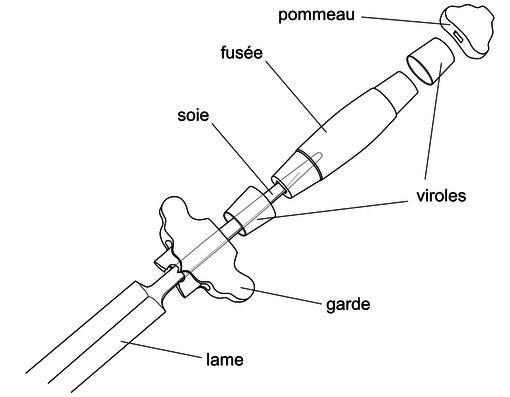
\includegraphics[width=0.69\textwidth]{../../Images/SwordParts/SwordPartsFr.pdf}
	\caption[Parties de l'épée]{Les parties de l'épée : La lame est prolongée par la soie sur laquelle sont emboités la garde, la poignée (fusée) et le pommeau. Les deux viroles sont deux anneaux de métal protégeant de l'éclatement les extrémités de la fusée. La garde protège la main portant l'épée. Généralement faite de bronze ou d'un métal similaire, elle est creuse et s'ouvre vers l'avant. La poignée, ou fusée, généralement faite de bois, a une forme de fuseau et est parfois recouverte d'un filigrane, de cuir, ou de peau de raie.
	Le pommeau, fabriqué dans le même métal que la garde joue un rôle primordial dans l'équilibre et le comportement de l'épée en contrebalançant le poids de la lame.}
	\label{fig:sword_parts}
\end{figure}

La principale particularité de la lame de l'épée chinoise tient dans ses deux tranchants quasiment parallèles. De 3 à 4 cm à la base, la largeur de la lame ne décroit que jusqu'à 2 à 3 cm près de la pointe, où les tranchants s'incurvent rapidement en une pointe acérée. 
Pour une lame de 70 à 80 cm, l'angle entre les deux tranchants est à peine discernable, à l'opposé de la forme franchement triangulaire de nombreuses épées médiévales européennes. 

Traditionnellement, la section de la lame pouvait être lenticulaire ou en losange avec une arête franche. 

Certaines lames pouvaient aussi comporter une gouttière, qui selon une légende tenace, aurait servi à permettre au sang de s'échapper de la plaie.
Une autre fantasmagorie au sujet de ces gouttières prétend qu'elles permettaient d'éviter à la lame d'être prise dans la blessure à cause d'un supposé phénomène de succion ou une hypothétique contraction des muscles blessés.
Je dois dire que j'ai de sérieux doutes sur la capacité d'un muscle entaillé à se contracter de manière significative autour d'une lame tranchante sans occasionner plus de dommages. Et en supposant qu'il le puisse, il n'y a aucune raison pour qu'une lame affûtée ne puisse pas s'ouvrir facilement un chemin vers la liberté.

La vérité est beaucoup moins fascinante : la gouttière permet d'alléger la lame sans compromettre sa solidité. \'{E}videmment, le moyen le plus facile pour réduire le poids de la lame est d'en diminuer l'épaisseur. Toutefois, la flexibilité de la lame en serait augmentée ce qui, au delà d'un certain degré, n'est pas souhaitable. Le profil des tranchants serait de même aplati, avec des conséquences possibles sur leur solidité. 
La gouttière autorise une lame plus légère avec un effet négligeable sur sa flexibilité et le profil des tranchants.
Par exemple, une gouttière de 1 cm de large et 2 mm de profondeur, sur deux tiers d'une lame lenticulaire de 75 cm représenterait un volume d'environ \unit{10}{\centi\meter\cubed}. La densité de l'acier étant de \unit{7,3}{\kilo\gram \per \deci\meter\cubed} à \unit{7,8}{\kilo\gram \per \deci\meter\cubed} selon sa composition et les traitements auxquels il a été soumis, une telle gouttière de chaque côté de la lame en aurait réduit le poids d'environ 150 g sans affecter le profil de ses tranchants. (voir figure \ref{fig:blade_section}) 
C'est loin d'être négligeable si on considère qu'une lame plus légère permet aussi d'alléger la garde et le pommeau. Ainsi, une telle gouttière permettrait au forgeron de monter une épée de 900 g, le poids habituel d'une épée chinoise historique, avec le même profil et la même longueur qu'une épée de plus de 1 kg sans la gouttière.

\begin{figure}[ht]
\centering
	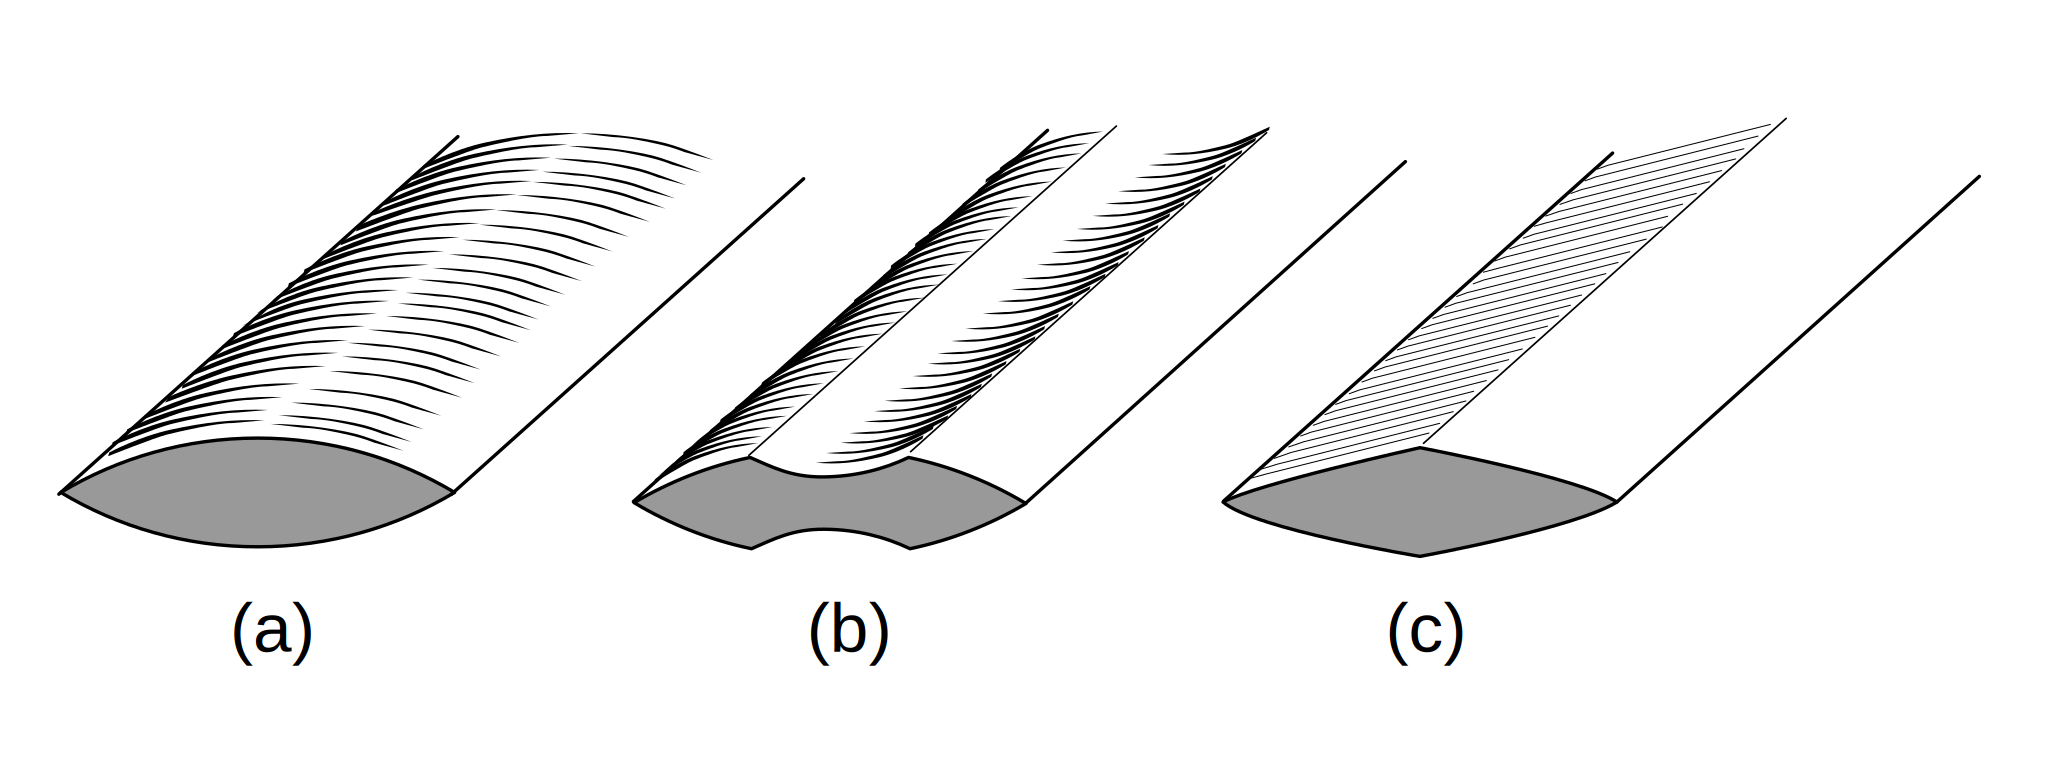
\includegraphics[width=0.69\textwidth]{../../Images/BladeSection/BladeSection.pdf}
	\caption[Sections de lame]{Sections de lames: (a) Lenticulaire. (b) Cette lame lenticulaire présentant une gouttière a le même profil de tranchants que la lame représentée en (a), mais elle est significativement plus légère grâce à la gouttière. (c) Losange.\\
	NB : pour des raisons de clarté, l'épaisseur des lames a été exagérée sur cette figure.}
	\label{fig:blade_section}
\end{figure}

Si le profil de la lame peut avoir une influence sur la durabilité des tranchants, le type d'acier dont la lame est faite affectera également leur solidité.
Avec un acier trop doux, les tranchants risquent de plier et de s'émousser après quelques coupes seulement. Pour durer les tranchants doivent être en acier durci, mais celui-ci étant cassant, il n'est pas envisageable de forger une lame exclusivement avec de l'acier dur. 
Un compromis est donc nécessaire entre la dureté de la lame, sa souplesse et son élasticité.

Notons bien qu'élasticité n'est pas synonyme de flexibilité : l'élasticité est la capacité de la lame à plier puis à revenir à sa forme d'origine. Si la limite d'élasticité est dépassée, la lame conserve une courbure ou se brise.
La lame doit être assez dure pour conserver des tranchants affûtés tout en étant suffisamment résiliente et élastique pour supporter des coups puissants et des chocs sans casser ni prendre une courbure définitive. 

En substance, l'acier est du fer additionné de 0,1\% à 2\% de carbone.  Il est aussi possible d'y allier d'autres métaux en faible quantité, comme le chrome, le nickel, le manganèse, etc.
La présence de ces éléments peut, malgré leur faible proportion, changer radicalement les propriétés mécaniques de l'acier conjointement avec les traitements par la chaleur.

Le \index{trempage}trempage est un processus consistant à chauffer la lame à haute température et à la refroidir rapidement par immersion dans de l'eau.
Suite à ce traitement, l'acier prend une structure cristalline particulière le rendant plus dur, mais aussi plus fragile.
D'autre part, comme il est impossible de refroidir instantanément et de manière homogène la totalité de la lame, le trempage crée aussi dans le métal des tensions persistantes qui risquent de fragiliser la lame.
Pour relâcher ces contraintes sans inverser les effets du trempage, il est possible d'appliquer à la lame un second traitement, appelé \index{recuit|see {revenu}}recuit ou \index{revenu}revenu. Il s'agit de chauffer à nouveau la lame à une température inférieure à celle du trempage avant de la laisser refroidir lentement, de manière à retrouver une bonne résilience. 

La technique appelée \index{trempage!trempage différentiel@\textit{trempage différentiel}}trempage différentiel constitue une alternative à ces deux traitements successifs. Renommée pour son utilisation dans la fabrication des sabres japonais, cette technique était à l'origine également utilisée en Chine.
Lors du trempage différentiel, seuls les tranchants sont soumis au choc thermique grâce à l'application d'argile sur la partie centrale de la lame, qui, ainsi protégée, conserve sa souplesse et son élasticité tandis que les tranchants sont durcis par le trempage.

Au Moyen-Âge en Europe, des tranchants d'acier durci étaient parfois soudés sur une âme en acier doux ou en fer. Autant que je sache, cette technique n'a été utilisée en Chine que pour les sabres.
La fabrication des épées droites chinoises faisait traditionnellement appel au procédé appelé \SanMei{}. La lame était constituée de trois couches d'acier soudées entre elles : une mince couche centrale dure formant les tranchants, entourée de deux couches d'acier doux ou de fer qui empêchaient qu'elle ne se brise sous des coups violents en donnant à la lame une structure élastique.

\section{Équilibre et propriétés dynamiques}
L'équilibre d'une épée est traditionnellement exprimée par la position de son 
centre de gravité (CG), aussi appelé centre d'inertie. Pour une épée de type \Jian{}, il se situe généralement entre 10 et 20 cm en avant de la garde, mesuré à partir de l'extrémité avant de la poignée.

Mais je pense qu'on donne habituellement trop d'importance à la position du CG. Bien que le CG joue un rôle important dans la manipulation de l'épée, il est loin d'être l'élément principal ayant une influence sur sa maniabilité. Alors que le CG d'un objet décrit son équilibre statique et comment il répond à l'application globale d'une force indépendamment de sa forme, les propriétés dynamiques de rotation dépendent aussi de la distribution des masses et de la forme. C'est la raison pour laquelle une barre et une boule homogènes ne se comportent pas de la même manière bien qu'elles aient toutes deux un CG confondu avec leur centre géométrique.

Les propriétés dynamiques d'une épée sont donc bien plus essentielles et déterminent la façon dont elle peut être maniée, comment elle bouge, comment elle tourne et répond aux actions exercées sur la fusée. En fait, il n'est pas rare de trouver des épées ayant un CG à la même distance de la poignée mais produisant des sensations radicalement différentes quand on les manipule.

Mais la mesure de la grandeur physique correspondant à ces propriétés dynamiques, le moment d'inertie, n'est pas particulièrement aisé, et une fois mesurée, l'interprétation de cette valeur scientifique en termes pratiques de manipulation d'une épée est loin d'être évidente.

Une façon précise de mesurer le moment d'inertie d'une épée est le test du pendule, qui consiste à en mesurer la période d'oscillation naturelle autour d'un axe situé à une distance donnée du CG. Après quelques calculs mathématiques, on obtient une valeur qui, pour être honnête, n'est guère parlante sans point de référence. De plus amples recherches seront assurément bienvenues sur le sujet.

Une manière plus simple d'observer les propriétés dynamique d'une épée est le test des points pivots. Bien qu'il soit bien moins précis, il a l'avantage de donner quelques indications sur la façon dont ces propriétés ont une influence sur la manière dont l'épée réagira aux actions exercées sur la poignée.

Pour réaliser ce test, tenez légèrement l'épée entre le pouce et l'index, et imprimez-lui avec légèreté une oscillation latérale. Vous pourrez remarquer dans la lame un point qui ne bouge pas : il s'agit du point pivot relatif à l'endroit où vous tenez la fusée (voir figure \ref{fig:pivot_points}).

Un changement de position des doigts sur la poignée déplacera le point pivot. En manipulant une épée, il est donc possible de contrôler la position du centre de rotation de l'épée en ajustant la position et la direction de l'action exercée par votre prise sur la poignée.

Les points pivots relatifs à la poignée se trouvent en général localisés dans la première moitié de la longueur de l'épée en partant de la pointe.

\begin{figure}[ht]
\centering
	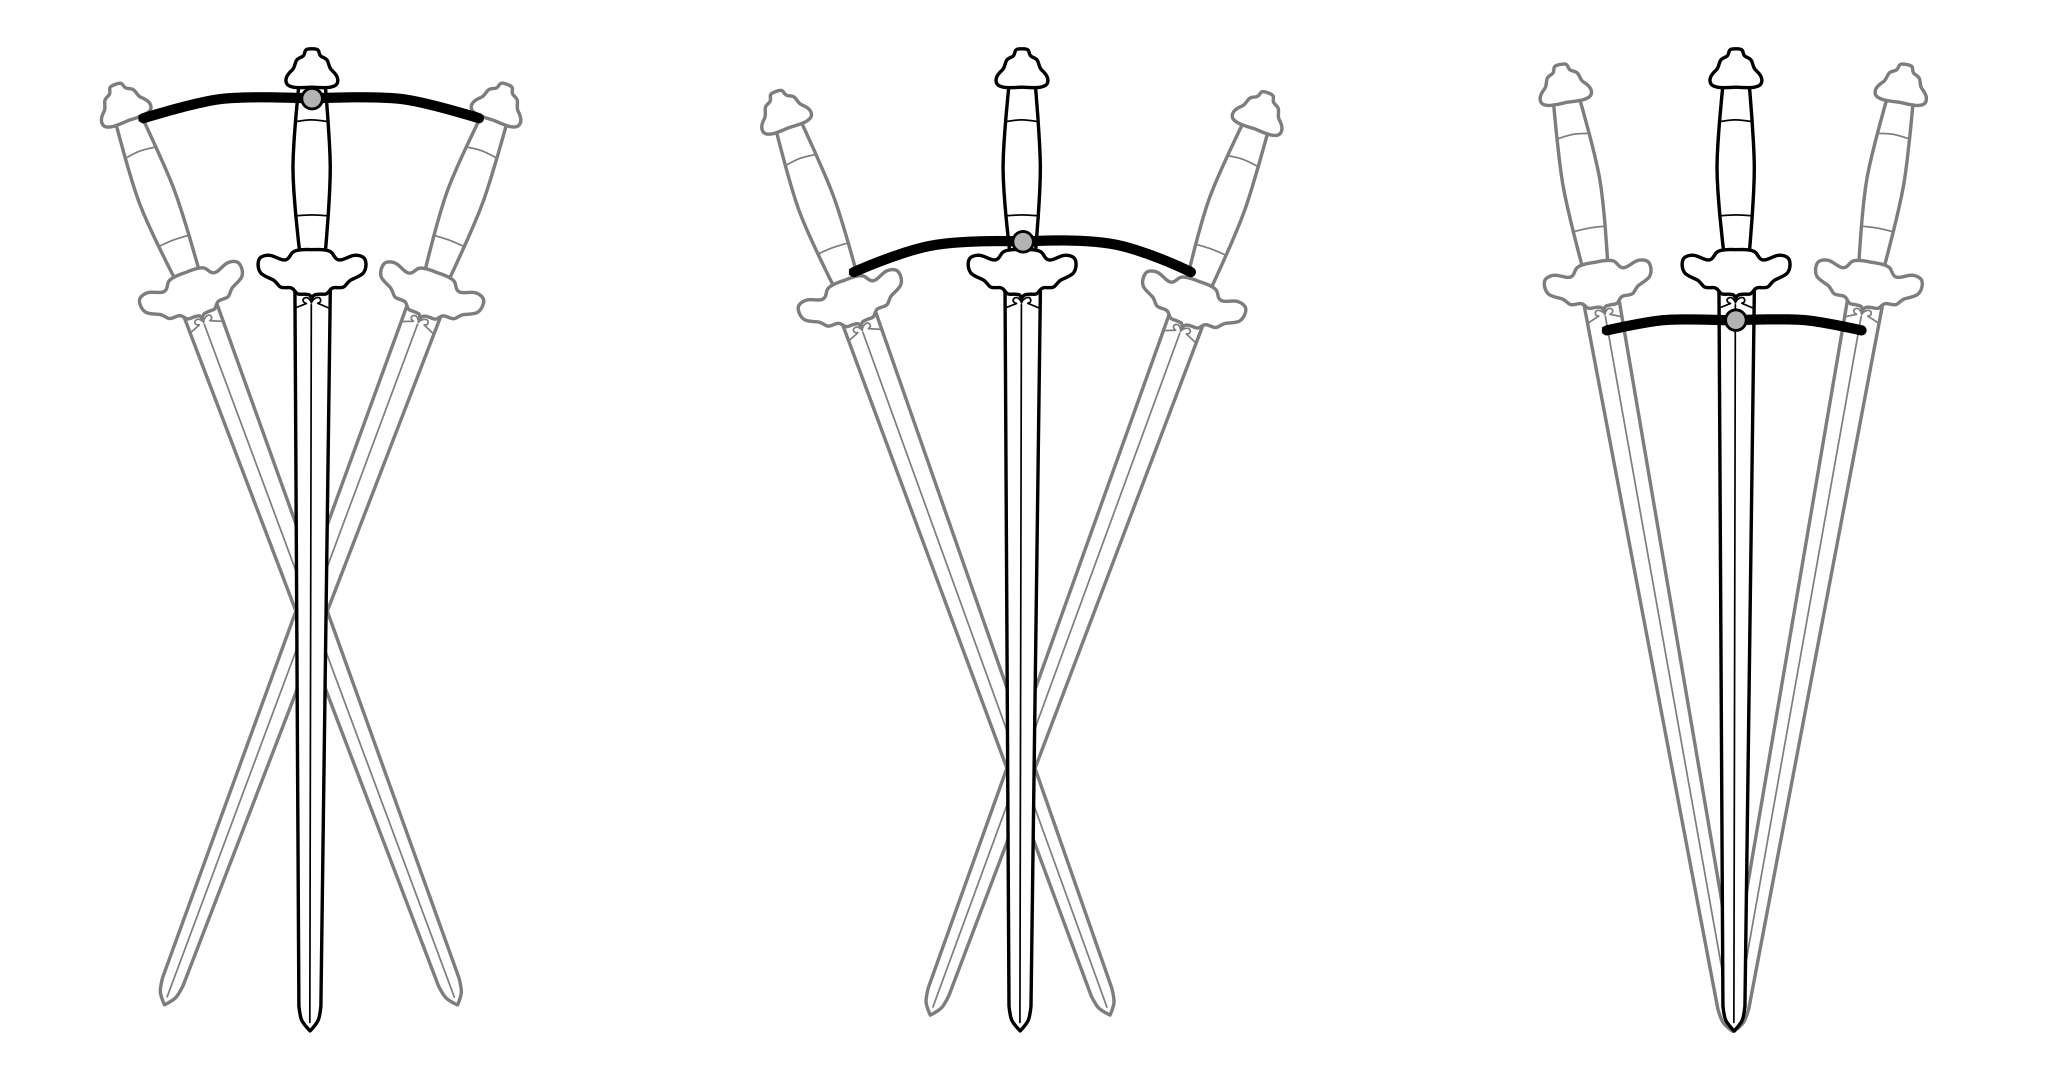
\includegraphics[width=0.80\textwidth]{../../Images/PivotPoints/PivotPoints.pdf}
	\caption[Points pivots]{Un point pivot est le centre de rotation naturel de l'épée selon l'emplacement et la direction d'une action exercée sur la fusée. Si l'épée est tenue près du pommeau et agitée latéralement, le point pivot est proche du centre de la lame (gauche). Tenir l'épée près de la garde déplace le point pivot plus loin vers la pointe (milieu). Pour placer le point pivot dans la pointe, une action latérale doit être exercée environ 2 cm en avant de la garde (droite). Bien que cela puisse sembler désavantageux, un ajustement approprié de la prise et une action oblique sur la fusée permet tout de même de contrôler ce point. De plus, il est ainsi possible de conserver sa pointe en ligne en tirant un estoc tout en contrôlant la lame de l'adversaire avec la garde.}
	\label{fig:pivot_points}
\end{figure}

Leur position est déterminée par la distribution des masses le long de l'épée et en particulier par les masses relatives de part et d'autre de la prise. Les facteurs affectant cette distribution sur une lame non fourbie sont la forme et les dimensions de sa section, comment elle diminue en largeur et épaisseur depuis la soie jusqu'à la pointe, ainsi que la taille relative de la soie. L'ajout d'un pommeau sur une lame non montée, même s'il est relativement léger, va modifier de façon importante la dynamique de l'épée. Non seulement le CG va se rapprocher de la garde, mais les points pivots vont être déplacés vers la pointe. Toutefois, un pommeau trop lourd risque de les déplacer trop en avant, voire même au delà de la pointe. \`{A} l'opposé, un pommeau trop léger rendrait difficile ou même impossible l'obtention d'un point pivot contrôlant exactement la pointe. 
Une amplitude correcte des points pivots permettant un bon contrôle de la lame nécessite donc un ajustement précis de la forme de la lame et des poids respectifs de celle-ci et du pommeau.

Le lecteur intéressé trouvera de plus amples informations sur ce sujet dans le livre \textit{Das Schwert \textendash{} Gestalt und Gedanke/The Sword \textendash{} Form and Thought} publié par le \textit{Deutches Klingen Museum} à Solingen. Bien qu'il ne présente exclusivement que des épées occidentales de différentes périodes, cet ouvrage présente une mine d'informations concernant l'équilibre et la dynamique d'une épée tout à fait applicable aux épées chinoises.

\section{Choisir une épée de \Taijijian{}}
%\subsection{Which sword for which practice?}
On trouve sur le marché une grande variété d'épées pour la pratique du \Taijijian{}. En choisir une est habituellement une affaire de goût et de budget.
Ces épées sont toutefois pour la plupart fort différentes des armes qui étaient encore en usage lorsque les formes traditionnelles de \Taijijian{} furent créées.
Beaucoup sont très approximativement équilibrées et sont soit trop légères ou trop lourdes.
Si le poids d'une épée d'entraînement n'est après tout pas si important et devrait être adapté de toute manière à l'expérience et aux capacités physiques du pratiquant, l'équilibre et les qualités dynamiques de l'épée ne devraient jamais être ignorées.
Assurer la sécurité des pratiquants d'exercices avec partenaire ou d'assauts libres constitue également une priorité absolue.

Il est probable que les pratiquants s'intéressant vraiment à tous les aspects du \Taijijian{} possèderont au final au moins deux épées, une pour la pratique de la forme, et l'autre pour les exercices avec partenaire et les assauts libres.

\subsection{Pratique de la forme}\index{forme!choisir une épée@\textit{choisir une épée}}
Comme les mouvements des enchaînements traditionnels étaient adaptés à l'équilibre des épées de l'époque de leur création, la pratique de la forme avec une telle arme, même passablement lourde, ne devait pas exiger d'effort particulier lorsque les principes du \Taiji{} étaient respectés.

Pratiquer de nos jours avec une épée de dimensions, poids et équilibre similaires à ceux d'armes historiques ne peut donc que nous rapprocher de l'esprit originel des formes traditionnelles.
Il est certes bien plus exigeant de manipuler une telle épée qu'une lame très légère, cela n'en est pas moins une occasion incomparable et stimulante d'approfondir notre compréhension de cet art et d'incarner les principes du \Taiji{}.

Cependant, bien qu'une épée lourde puisse être un meilleur guide qu'une épée légère pour la pratique de la forme, elle laisse aussi moins passer les erreurs techniques et l'excès de tension musculaire.
Le poids de l'épée devrait donc être adapté à l'expérience du pratiquant et à sa forme physique. Il n'est pas judicieux pour un débutant de pratiquer avec une épée tellement lourde qu'elle ne pourrait que sanctionner ses articulations et ses muscles au moindre mouvement incorrect qu'il ferait.
Ainsi, une épée de bois ou d'acier bon marché conviendra parfaitement pour débuter et mémoriser la forme, mais deviendra vite limitante pour un approfondissement de la pratique.
Lorsqu'il aura acquis une expérience suffisante, le pratiquant aura tout avantage à passer à une épée correctement équilibrée et d'un poids approximatif de 700 à 900 g, équivalent à celui d'armes historiques.

De même, les débutants apprenant la forme et les bases risquent d'être gênés inutilement par une longue lame et devraient favoriser des épées plus courtes. Les pratiquants avancés, si leur prise est vraiment relâchée, devraient toutefois être capables de s'accommoder aisément d'une lame plus longue, à condition que sa longueur ne soit pas excessive.

Une règle classique consiste à déterminer la bonne longueur de lame en tenant l'épée verticalement le long du bras gauche, comme pour l'ouverture de la forme. La pointe de la lame devrait alors se trouver en face de l'oreille. En résumé, ceci est tout à fait équivalent au fait de s'assurer que la lame est en moyenne plus longue que la longueur du bras de la plupart des adversaires potentiels. Ceux-ci ne pourraient ainsi pas se protéger d'un estoc en le bloquant au niveau de la garde.
Quoiqu'il en soit, une lame de 70 à 75 cm devrait convenir à la plupart des pratiquants.

La présence d'un \index{pompon}pompon dépendra du style pratiqué. Certains styles en utilisent un, d'autres pas, à l'instar du \Yangjia{} \Michuan{}. 

On a dit beaucoup de choses sur le rôle du pompon. Il est largement admis que, pendant la pratique de la forme, la manière dont le pompon bouge donne des indications sur la qualité de mouvement du pratiquant.
Je suis prêt à accepter cet argument qui fait du pompon un outil pédagogique pour équilibrer l'intention entre la pointe de l'épée et la poignée. Mais si le pompon accapare trop l'attention du pratiquant, celui-ci risque fort de finir par pratiquer une forme de pompon. 

Je suis bien moins convaincu par d'autres explications telles que l'utilisation du pompon pour détourner l'attention de l'adversaire. Je préfère personnellement menacer l'adversaire avec la lame, qui est bien plus impressionnante et qui, contrairement au pompon, est tranchante et ne peut pas être saisie.

En réalité, si on se réfère aux représentations historiques d'épées et de bretteurs, il semble que le pompon soit d'une invention assez récente. Je penche pour une évolution décorative des dragonnes qu'on peut voir sur des images plus anciennes et qui servaient à assurer l'épée dans la main pendant le combat.
En tout état de cause, n'utilisant pas de pompon, je ne peux que suggérer de faire à ce sujet ce que recommande votre style.

\subsection{Exercices avec partenaire et applications martiales}\index{exercices avec partenaire!choisir une épée@\textit{choisir une épée}}\index{applications martiales!choisir une épée@\textit{choisir une épée}}
Il est possible de pratiquer avec la même épée que la forme, des exercices simples avec partenaire tels que les épées collantes, guider et suivre, etc. tant qu'il n'y a aucune attaque lancée au visage ou vers la partie supérieure du corps.

Je recommande toutefois vivement de réserver les exercices sans protections strictement à des pratiquants expérimentés et entraînés, ayant l'habitude de pratiquer ensemble. Dans tous les autres cas, l'utilisation d'une épée conçue pour le travail avec partenaire et des protections adéquates  \textendash{} au minimum un masque d'escrime et des gants \textendash{} est absolument nécessaire pour réduire les risques d'accident.

Des épées rigides non tranchantes dont la pointe a été recouverte d'une pièce de cuir peuvent constituer un bon compromis pour un budget limité. Toutefois, il faut garder à l'esprit que ces épées n'ont pas été conçues pour cet usage et qu'elles peuvent s'avérer dangereuses sans les protections et précautions adéquates. Un accident est toujours possible, et quiconque utilise de telles épées pour un travail avec partenaire le fait à ses propres risques. Notez bien qu'il n'est pas recommandé d'utiliser ici ce qu'on appelle une lame flexible. Non seulement ces lames ne sont pas adaptées au travail avec partenaire, elles sont aussi tellement fines qu'elles en sont presque tranchantes.

Contrairement à ce qu'on pense généralement, les épées de bois ne sont pas réellement plus sûres puisqu'en raison de leur rigidité, elles ne peuvent absorber efficacement le choc d'un estoc. De plus, l'épaisseur de lame des épées de bois interdit une bonne sensation du contact.

La meilleure option reste assurément l'utilisation d'épées conçues spécialement pour le travail avec partenaire. Leurs tranchants épais et arrondis ainsi que leur pointe retournée les rendent relativement sécurisées à condition de porter au minimum un masques d'escrime et des gant rembourrés. Une veste d'escrime rembourrée apportera une protection supplémentaire permettant des exercices plus intenses et dynamiques. 
D'autre part, avec un poids supérieur à 800 g, elles autorisent moins que des épées légères les entorses à une réalisation correcte des techniques dans le respect des principes, ce qui doit être vu comme un avantage dans la perspective des applications et exercices techniques.



\subsection{Assaut libre}\index{assaut libre!choisir une épée@\textit{choisir une épée}}
Bien qu'on puisse pratiquer des jeux doux et tranquilles avec des lames non protégées ou des épées mouchetées à l'aide d'une pièce de cuir, je recommande vivement de toujours utiliser des épées spécialement conçues pour l'assaut libre (\textit{sparring}) et des protections appropriées pour la pratique de l'escrime (masque d'escrime, gant rembourrés, veste d'escrime rembourrée).
Sans protections efficaces ni précautions, même en restreignant volontairement les attaques aux parties basses du corps, des réactions instinctives peuvent être la cause d'accidents aux conséquences graves. 

Les épées de bois ne sont pas plus adaptées aux assauts libres qu'aux exercices avec partenaire. Des coupes vigoureuses et non contrôlées heurtant les doigts ou un os ne sont pas moins douloureuses ou dangereuses qu'avec une épée en acier. Sur un estoc, au contraire d’une lame d’acier, une épée de bois ne plie pas et toute l’énergie du choc est transmise à la cible au lieu d’être partiellement dissipée par la lame.

Une bonne épée pour l'assaut libre doit avoir une pointe arrondie ou retournée et des tranchants épais et arrondis pour permettre des estocs et coups de taille moins dangereux. Elle doit être suffisamment lourde pour obliger à utiliser des techniques correctes et empêcher des mouvements de poignet irréalistes similaires à ceux utilisés en escrime moderne au fleuret. Cependant, son équilibre doit permettre de réaliser toutes les techniques des formes traditionnelles de \Taijijian{} de manière naturelle avec des transformations vivaces et aisées.

Il existe maintenant des épées chinoises en acier conçues pour l'assaut libre et les exercices avec partenaire. Mon modèle favori, et celui que nous utilisons dans notre groupe, est produit par \textit{Péter Regenyei Armory}. Cette épée pour l'assaut (sparring \Jian{}) est le résultat d'une collaboration entre Mattias Nyrell, instructeur principal de \Jianfa{} du \textit{Historisk Fäktning i Linköping}, Péter Regenyei, forgeron renommé fabricant d'épées, et Peter Dekker, un antiquaire spécialisé dans les armes et armures de Chine et autres régions d'Asie, fondateur de \textit{Mandarin Mansion}.

La conception de cette épée s'inspire d'une \Tuanlianjian{} historique appartenant à la collection privée de Peter Dekker. Ces épées modestes et pratiques sont aussi connues sous le nom d'épées de milice puisqu'elle étaient probablement utilisées par des milices rurales pour défendre leurs biens et leurs villages. L'aspect des épée pour l'assaut de Péter Regenyei contraste donc fortement avec le style doré et parfois ampoulé de la plupart des épées chinoises sur le marché. Cependant, par leur simplicité, ces épées reflètent la beauté et la qualité de leur fabrication artisanale.

La lame de 73 cm de long aux bords presque parallèles possède une pointe retournée, une section en diamant aplati et des tranchants arrondis et épais de 1 à 2 mm. Ces bords épais et la pointe retournée assurent une bonne répartition de l'énergie dans les coupes et les estocs sur les protections. Cela ne constitue toutefois pas un sauf-conduit pour des coupes ou des estocs appuyés de toute force. En effet, bien que cette lame ait un certain degré de flexibilité, elle n'en est pas moins assez rigide et il peut être judicieux de porter un plastron, surtout pour les femmes, et un gorgerin en plus de la veste rembourrée habituelle.  

Malgré un poids de 800 à 900 g, cette épée semble plutôt légère dans la main, avec une forte sensation d'homogénéité du pommeau à la pointe. Le seul point qui pourrait demander un peu d'habitude est la section anguleuse de la poignée. Mais ceci peut en fait s'avérer un avantage en assaut libre pour mieux sentir l'alignement de la lame en portant des gants rembourrés.

Son excellent équilibre en fait une épée vivace et agile, très aisée à contrôler à condition d'être correctement connecté et de la mouvoir avec tout le corps et pas uniquement à partir du poignet ou du bras. Tous les mouvements et leurs transformations semblent naturels et dynamiques, que ce soit en déroulant la forme \Kunlun{} du \Yangjia{} \Michuan{} ou en assaut libre.

Je ne puis donc que recommander le pratiquant de \Taijijian{} passionné d'investir dans ce modèle d'épée. Pour tout dire, si vous ne deviez posséder qu'une seule épée, ce serait celle-ci: elle est en effet parfaite non seulement pour l'assaut et le travail avec partenaire, mais aussi pour la pratique de la forme.

% !TeX spellcheck = en_GB
\chapter{\Taijijian{} practice}
\Taijijian{} is the pinyin transcription for the Chinese word designating the art of the sword based on the \Taiji{} principles \textendash{} also known as the \Taiji{} (or Taichi) sword \textendash{}  and studied together with \Taijiquan{}, the \Taiji{} boxing.

In most styles, \Taijijian{} practice consists essentially, if not exclusively, in learning and performing a sword form.
As such, it complements bare hand practice and provides the practitioners with an invaluable tool to improve their skills.
The sword is indeed a devoted partner, always ready to guide us on the way towards a better understanding and embodiment of the \Taiji{} principles.

However, I am convinced that, in this respect, \Taiji{} sword practice can only benefit from the thorough study of basic techniques, fencing notions, partner drills, martial applications and even free play.

In the XXI\textsuperscript{st} century, \Taiji{} fencing does not have to be practical any more: fighting skills and efficiency are not sought for themselves, but their purpose is nothing but the application of the \Taiji{} principles in action. From basic techniques to free fencing, the practitioners will strive to achieve unity with their sword, improve their nimbleness and sensitivity, relax their body and mind, develop their \Yi{}, etc. 

Last but not least, this life-long endeavour should also bring its share of fun.

\section{\index{basic exercises}Basic exercises and \index{warm-up}warm-up}
The goal of warm-up and basic exercises is the preparation of the body and the mind to the safe performance of efficient techniques conforming to the \Taiji{} principles.

Warm-up should gently mobilise the joints and muscles to bring them to their optimal functioning level for smoother movements and lower risks of strains.
An emphasis on the upper body is necessary, in particular the shoulders, arms, wrists and fingers, which do most of the job of sustaining the sword.
But the lower body should not be overlooked in preparation to the footwork which is of crucial importance in fencing.

I usually tend to start the warm-up by mobilising the pelvis and the spine, which are at the core of every movement in \Taiji{}, and then continue with the shoulders, elbows, fingers and wrists.
For the lower body, I start with the ankles, carry on with the knees and then the hips, exercising balance at the same time.
Eventually, the session ends with codified and free footwork.

Before proceeding to basic techniques, it might be a good idea to finish the warm-up session using the sword as an accessory.
This will not only serve to further stretch the wrists and shoulders, it will also help the practitioners to exercise their relationship with the sword.
The repetition of a simple non-technical movement helps indeed to install the relationship between the sword and the body: the sword's energy, absorbed and concentrated in the body, is returned to the sword for the next movement\footnote{See chapter \ref*{ch:grip} for more details on handling the sword.}.

Repetition is of crucial importance as well for practising basic techniques, the emblematic basic cuts and thrusts. Repeating them in series is essential to technical precision and body control, requisite conditions for the proper realisation of techniques in less controlled situations.

It is interesting as well to practise the basic techniques with \index{target}targets, not only to exercise precision, but also to develop the mindset and relaxation of the body appropriate for an effortless efficiency of techniques.
For \index{thrusts}thrusts, \Ci{} or \Zha{}, cloth-pegs hung on a string at throat level make pretty convenient targets.
Targets for \index{cuts}cutting techniques are more difficult to set up: cuts are supposed to pass through the target, hence hard resisting targets are out of question. Non ligneous plant stalks or a slab of clay can make appropriate cheap targets for test cutting without requiring a dangerously sharp blade. Clay works quite nicely with a regular blunt sword, but do not use your favourite one or be prepared for intensive cleaning of your sword after the session. Make sure as well that clay does not get soiled with pebbles or sand to avoid damaging the blade.

Those exercises build up the basics which in combination constitute the source of all the techniques that can be practised in the more diverse context of the form.


\section{\index{form!practice@\textit{practice}}Form practice}
The form is a set of movements arranged in a continuous succession of techniques which some practitioners present as a mock fight with an imaginary opponent.

However, I personally think that this is not the complete story: although the movements of the form are martial techniques indeed, the whole set does not constitute a single combat from start to end. Techniques are rather arranged in short series, which the European tradition calls 'pieces', describing a variety of situations where these techniques may be applied. Variations are given throughout the form and as most movements may have several applications, series may overlap or describe varying situations.

The form is much more than a catalogue of techniques, it is the source from which all applications proceed according to the infinity of possible situations. As an actualisation of the \index{YinYang@\Yin{}/\Yang{}}\Yin{}/\Yang{} principle issuing from the \Taiji{}, the \Taijijian{} form contains all the potentialities for the generation of countless applications. Performing the form is thus generating a potential for infinite creativity, reserving the practical expression of techniques for their application in real situations.

In my opinion, the form is therefore essentially a tool for achieving a better understanding and embodiment of the \Taiji{} principles. 
Memorisation is only a beginning: what is truly trained when practising the form is \index{YinYang@\Yin{}/\Yang{}}\Yin{}/\Yang{} \index{transformation}transformation and directing the \index{Yi@\Yi{}}\Yi{} as a continuous yet ever-changing flow.
Gradually, with practice, unity with the sword can be achieved, the form becomes more and more internal, gains in fluidity, feels easy and natural. 
Until ultimately, I like to think that the body and the mind are delivered from all their tensions, and nothing remains but pure \index{Yi@\Yi{}}\Yi{} effortlessly generating the form.

The form, however, is not only a mental exercise but it also physically trains the body.
Some movements have indeed an exaggerated amplitude to develop strength, balance and flexibility.
Others are clearly intended to be spectacular and demonstrative. 
Every \Taijijian{} form is thus made of a mixture of internal martial training, gymnastic exercise, and spectacle.
Discerning how these characteristics are actually expressed in the different movements allows the practitioner to favour at will one aspect or the other.

To those interested in improving their fencing skills, the form provides an invaluable tool for building a strong repertoire and knowledge of martial techniques while practising the body mechanics appropriate for their effective application.

The form, however, is not strictly representative of the occurrence of techniques in free fencing, where the most frequent and effective ones are rather simple.
The form contains surprisingly complex movements that may contribute to its demonstrative character, but probably also prepare the practitioner to master extreme techniques appropriate to exceptional circumstances.  
Most swordsmen of the time might well have never needed to put these techniques to practice, those who actually had to might have owed their life to this preparation instead of having been overwhelmed by a stunning situation.

In modern times, martial efficacy of \Taiji{} fencing is not a matter of survival any more, but, within the context of friendly controlled practice, aims more readily at freeing the mind and the body from their tensions.
The martial interpretation of the form thus provides a whole range of situations where the practitioners may put their body and mind to the test in partner drills and martial applications.

\section{\index{two-person drills!practice@\textit{practice}}Two-person drills and \index{martial applications!practice@\textit{practice}}martial applications}
Two-person drills are simplified and codified situations whose goal is to introduce and exercise important principles and notions of \Taiji{} fencing such as distance and time, the lines, sensing through the blade, footwork in response to the opponent's moves, nimbleness, etc.
Entirely dedicated to this pedagogic goal, those drills are essentially continuous exercises or games, most of the time without much concern for the realism of the situations.

Martial applications will then develop the same principles and notions within a codified or semi-codified simulated piece of fight, simultaneously giving examples of the potential practical use of techniques from the form.
As such, they open the way to a better understanding of the form, highlighting the   martial essence of movements and the distinction between practical and demonstrative moves.

Although martial applications may be much more realistic than two-person drills, it must be acknowledged that they none the less are simulations far from reproducing exactly all aspects of a true sword fight to death.
Depending on their experience and protection level, practitioners may perform the applications at different speeds or may be more or less well-disposed towards their partner, thus achieving different levels of realism. 
Some applications may work well at low speed, with caring partners but not any more when performed faster, with partners who do not hold their attack. 
Performing applications with full \index{protective gear}protective gear which allows full blows may thus be more demanding and what used to be working with less protections and more precautions might not work as nicely.
On the contrary, performing an application at low speed may allow a non-cooperative partner to counter-attack whereas such a riposte would have required light-fast reactions against a technique performed at full-speed. 

Evaluating the true effectiveness of martial applications needs therefore to account for all those factors.
For what is worth, as far as they allow us to develop and practise the \Taiji{} principles and fencing notions, the approximate realism of martial applications should give entire satisfaction for our purpose. The efficiency of an application should be only a consequence of our conformance to the principles, and definitely not a matter of speed or strength.
Thus, martial application practice may help develop the proper mindset and body disposition for the effective application of techniques and principles in free play.

\section{\index{free play!practice@\textit{practice}}Free play}
Free play refers to the wholly non-codified simulation of a sword fight.
Depending on the protective gear worn by the practitioners and their experience, rules may be defined to guarantee their safety.
In any case, violence is definitely ruled out and free play should always remain a friendly game, without any overly competitive mind.

I understand that some practitioners may feel concerned that free play might possibly not be considered as internal.
Actually, expressing martial techniques should not be confused with external practice. 
My personal view is that we may speak of \index{internal practice}internal practice as long as every movement is born from the \index{Yi@\Yi{}}\Yi{} which shapes the technique and, originating from the centre, is eventually expressed towards the periphery. Efficient techniques proceed naturally from the appropriate intention and a relaxed body, well mastered principles that have become natural and can thus be applied spontaneously.
Students of internal arts should not cling too much to trifling technical details, which are only the finger of the wise man. 
They should reach for the moon: develop their capacity to apply the principles in challenging and unpredictable situations.\footnote{To be honest, I do not even think there are that many differences between internal and external arts when it comes to high level practice. The main difference would rather lie in the way these arts are taught. External arts first focus on techniques and let the student figure out the principles whereas internal students are taught the principles and must figure out how to perform the techniques in conformance.} Everything else should follow.

Nimbleness of the \index{Yi@\Yi{}}\Yi{} and of the body results from an open and free, tensionless mind allowing us to remain relaxed when facing the threats of an opponent.
After all, this may be the true practical application of martial arts in our modern times: not to let ourselves overwhelmed by stress in all matters of urgency.

Of course, as already mentioned above, technique efficacy is entirely relative to the context: free play is \textendash{} and must stay \textendash{} no more than a simulation that cannot reproduce all aspects of a true sword fight, and in particular the psychological aspects.

In any case, nowadays, arguments are not settled any more in duels or sword fights and the purpose of \Taiji{} fencing is more a matter of personal development than of actual fighting capacities. Our main concern is not to hit the opponent by all means but to do it with the appropriate manner while not being hit. How the goal is reached is more important than the goal itself: scoring a hit against an opponent should be the result of the proper application of the \Taiji{} principles to the current situation, and not a purpose in itself.

Thus, in order to avoid excessive competition,  I prefer not to count hits and only appreciate subjectively the quality of the actions. Taking videos of free play sessions may also help reviewing actions afterwards to highlight the positive and the negative. 
With really nothing at stake, this less competitive approach allows to focus more on the principles and internal practice and limits the risks of accidents.

\fiche{
Not quite sure about the following, should be confirmed before including it:
This goal revives somehow the Neo-Confucean ideal of self-cultivation which arose during the \Ming{} dynasty and was expressed by the literati, among other things, in their perception of martial arts.
}

\fiche{
\section{Internal vs. external}
    movement coming from the centre, associated with yi which will shape the technique, expression towards the outside. should not attach too much importance to technical details which are only a consequence of the correct performance and application of principles, being relaxed and guiding from the centre with the yi but adapted to external energy, link and sensitivity.
    external does the opposite, the technique us guided by the periphery of the body.
        
}

\section{\index{safety}Safety considerations}
The practice of \Taiji{} has been associated with health and personal development for perhaps over a century now. We could thus expect that preserving a good health should go along with the preservation of our physical integrity, and that \Taijijian{} practice could be taken rather safely, from solo form to free play.
Actually, even hard training of warriors in the past may have presented some degree of safety: what would have been the point of decimating the troops before actually sending them to battle. 

Of course, accidents sometimes happen, but there is no reason why they should be the norm. We should in all circumstances bear in mind that even a blunt sword can be a deadly weapon and we should behave accordingly. 
Safe practice actually results from the combination of a responsible attitude with the appropriate equipment. 
The mind-set we adopt during any kind of practice is most important indeed. It is essential to me that we feel responsible not only for the physical integrity of other people around us when we hold or wield a sword, but also for our own safety. 
The first consequence of this state of mind is that, if it is adopted by all practitioners, everyone constantly maintains a good degree of watchfulness instead of solely relying on others for their safety.
Furthermore, if we ever get hurt despite all precautions, this attitude also prevents us from systematically blame others for it.

It is also important to remember that solo practice is not exempt from danger. Our concern for safety must not be limited to the practice ground but starts in the changing-room. As soon as we start holding or wielding a sword,  we must do so most carefully. When carrying a sword, its blade should be held vertically along the arm or its tip should be pointing to the ground. Never ever wave a sword heedlessly and always make sure to be at safe distance from other people before starting to practise. 

When it comes to \index{two-person drills!safety@\textit{safety}}partner drills, \index{martial applications!safety@\textit{safety}}applications or \index{free play!safety@\textit{safety}}free play, we should always adapt the speed and intensity of the practice to the less advanced partner and to the protective gear. 

Both partners should use the same kind of equipment: a blunt sword\footnote{See chapter \ref*{ch:chinesesword} for more details.} and a \index{protective gear}fencing mask are a minimum. Gloves and a padded jacket allow more dynamic practice and are highly recommended for free play. 

If the above advices are followed, the risks of accident may be kept at a minimum. However, it should be always remembered that there is an inherent risk to any martial practice, that accidents can happen, and that when they do, the only thing we can do is to minimise as much as possible their consequences with the appropriate equipment and attitude. Those who partake in \Taijijian{} fencing should acknowledge this idea and accept that they do so at their own risk. 

\fiche{ keep some sense of responsibility for any incident that may happen
 and urges us to seek the mistake in our acts first. We may thus always learn lessons from accidents and keep a friendly spirit with other practitioners. 
}

\fiche{
Maybe use the following in the chapter about handling the sword.

no constraint on the sword, leverage the weight and inertia of the sword to move it.

Li strength vs Jin force, Jin is a the use of the whole body to express strength in a connected and tensionless manner. 
Require awareness of the situation: position, direction and movements of the sword, to be able to adjust and move it without tension.

\Taiji{} insists on not using muscular strength (actually not more than required to stand and hold the sword) Chinese uses the \Li{} word (physical strength, strive) as opposed to {J\`{\i}n} (physical strength as well, but vigour, expression, energy), 
\Li{} seems to be less subtle than {J\`{\i}n}
It is important to note at this point that the connection between the body and the sword is indeed a two-way relationship. While it is true that one's sword should become an extension of one's arm, this claim is basically of no help at all to most {T\`{a}ij\'{\i}j\`{\i}an} beginners who desperately try to figure out how to cope with a 30-inch-long blade. I have found much more informative to liken the sword to a dancing partner. 
    In the same way, a good sword player should make her or his sword look as if it were alive, with graceful and fluid movements. There should be no hard constraint placed upon the sword, nor should the body be strained in any way by the sword inertia. 
This can only be achieved by a constant awareness of the sword position and movements and by a good relaxation allowing to absorb the energy back from the sword and perform the next move accordingly. become one with the sword (corollary of sword being an extension of body and principles: body is united)
 
}

\part{Notions élémentaires}
% !TeX spellcheck = fr_FR
\chapter{Prise et manipulation}\label{ch:prise}

\paragraph*{}
Dans la culture chinoise, l'escrime et la calligraphie sont des formes d'art intimement liées et on entend communément dire qu'il faut tenir une épée comme s'il s'agissait d'un pinceau de calligraphie.
Cette affirmation semblera claire à quiconque s'est essayé à la calligraphie chinoise : pour parvenir à un bon contrôle du tracé, le pinceau doit être tenu fermement mais sans tension de manière à être relié au centre du corps du calligraphe.
La moindre faiblesse ou tension dans la prise du pinceau aura pour conséquence des traits anguleux ou hésitants.

De même, en manipulant une épée, toute tension ou faiblesse de la prise s'opposera à la fluidité des mouvements et à une connexion correcte entre l'épée et le corps, se traduisant invariablement par des mouvements d'épée maladroits et sans vie.
Pendant les assauts libres, une prise incorrecte empêche de ressentir, de s'adapter et de réagir efficacement aux mouvements de l'adversaire.

La manière de tenir la fusée déterminant la capacité à contrôler l'épée, une saisie correcte, un alignement adéquat et une attitude exempte de tensions sont les éléments fondamentaux permettant de réaliser une bonne unité avec son épée.

\section{La prise de l'épée}
De toutes les prises que j'ai pu expérimenter, je recommande particulièrement celle représentée sur la \index{prise} figure \ref{fig:prise} tant pour la pratique de la forme que pour l'assaut libre.

Pour prendre l'épée en main, alignez la gueule du tigre, le poignet et l'avant-bras dans le plan de la lame puis saisissez la partie médiane de la poignée, entre les deux viroles.
Le pouce verrouille la prise au centre de la fusée en se refermant sur l'extrémité du majeur et de l'annulaire.
L'index et l'auriculaire restent libres, participent au contrôle précis de la position de la poignée dans la main et permettent de relâcher ou resserrer la saisie.

\begin{figure}[ht]
	\centering
	\subfigure[]{\label{fig:prise}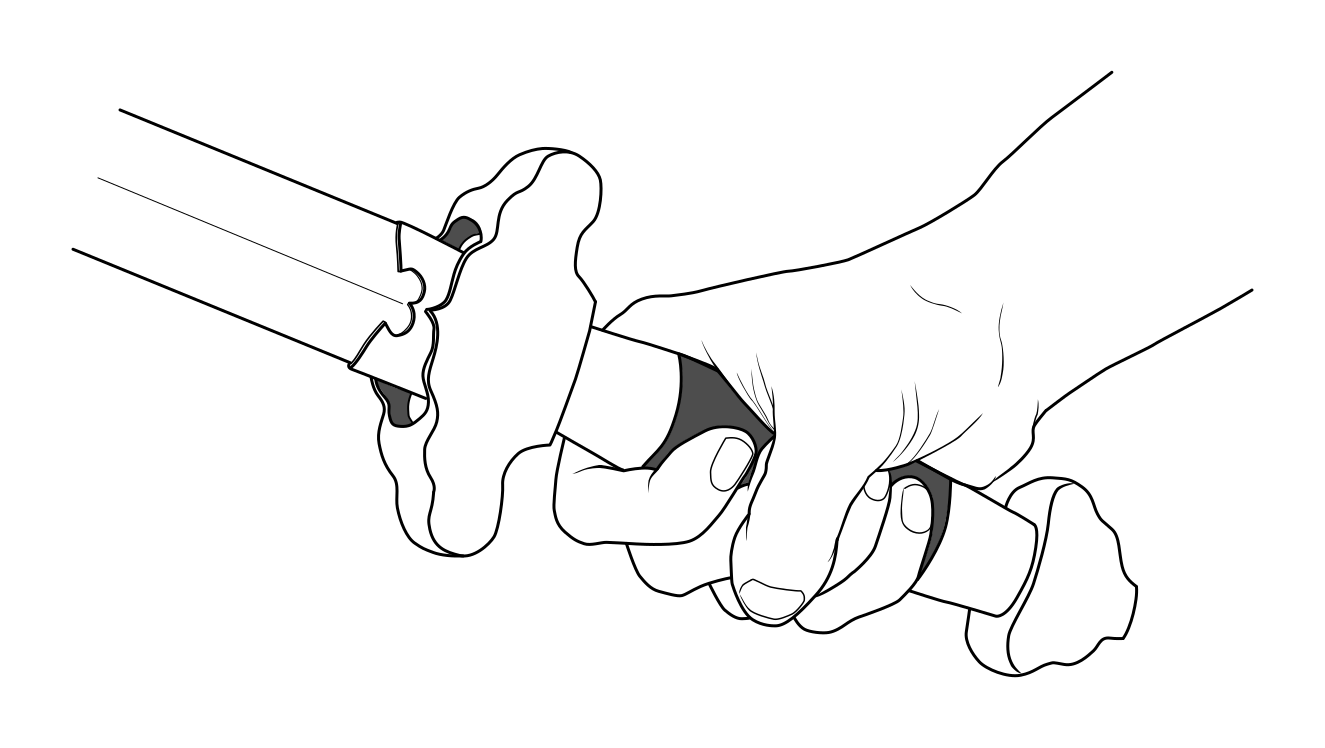
\includegraphics[width=0.69\textwidth]{../../Images/SwordGrip/sword_grip.pdf}}
	\subfigure[]{\label{fig:alignement}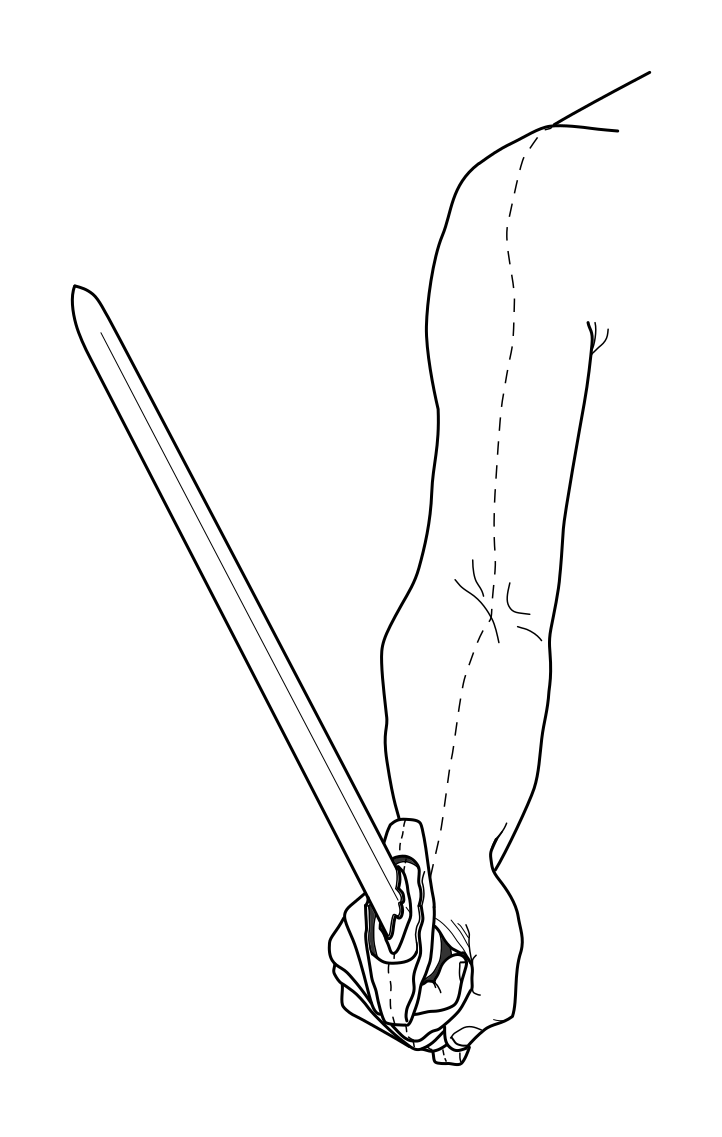
\includegraphics[width=0.29\textwidth]{../../Images/SwordGrip/alignment.pdf}}
	\caption[La prise de l'épée]{La prise de l'épée: \subref{fig:prise} la main saisit la poignée en son milieu, le pouce recouvrant le majeur et l'annulaire;
	\subref{fig:alignement} les articulations du poignet, du coude et de l'épaule sont alignées avec la lame de l'épée ainsi que représenté par la ligne en pointillés.}
\end{figure}

Comme le montre la figure \ref{fig:alignement}, le poignet, le coude et l'épaule sont situés dans le même plan que la lame.
L'épée est ainsi solidement enracinée dans la main et les centres de gravité de l'épée et du corps sont connectés, une condition essentielle pour une absorption et une expression efficaces, sans aucune tension ni contrainte sur les articulations, les muscles et tendons.
De plus, dans cette position, le coude est situé à l'intérieur de la zone de protection de la garde et ainsi, est moins exposé à des touches rapides.

\`{A} l'occasion, il est possible d'ajuster la saisie pour réaliser une technique particulière, mais il est essentiel dans ce cas de prendre garde à ne pas rigidifier ni affaiblir inconsidérément la saisie de l'épée.
En tout état de cause, lorsque les circonstances ne sont pas favorables pour un changement, ce qui est bien souvent le cas en assaut libre, il est préférable de s'en tenir à la prise principale présentée ici.

La mobilité de l'épée est également contrôlée par le resserrement ou le relâchement de la saisie. 
Il est important toutefois de garder à l'esprit que les doigts ne doivent jamais lâcher totalement la fusée : même en réalisant un moulinet, tous les doigts doivent constamment maintenir un certain contrôle de la poignée. 

Je suis convaincu qu'il est primordial de résister à la tentation de saisir la poignée au plus près de la garde, même si, la prise étant alors plus proche du centre de gravité de l'épée, celle-ci en semblerait alors moins lourde.

Tout d'abord, outre le fait que la forme en fuseau de la poignée est parfaitement adaptée à une prise centrée, dans cette prise, la garde et le pommeau sont suffisamment éloignés de la main pour ne pas gêner les mouvements de l'épée.

De plus, les gardes chinoises étant très étroites et n'enveloppant pas totalement la main comme le fait la coquille d'une rapière, elles protègent moins la main armée.
Toutefois, grâce à la position centrée de la prise, en contrôlant la lame adverse avec la garde, le pouce et l'index sont plus éloignés de la menace du tranchant adverse et donc moins exposés à des coupes fortuites que si la main est proche de la garde.

Enfin, avec une épée correctement équilibrée\index{equilibre@équilibre}, le centre de rotation résultant de cette prise centrée est précisément localisé à l'endroit permettant au pommeau de jouer pleinement son rôle dans l'équilibre dynamique de l'épée\footnote{Voyez le chapitre \ref*{ch:epeechinoise} pour de plus amples détails sur l'équilibre.}, ce qui garantit des mouvements vifs et rapides qui feront réellement la différence en assaut libre.

\section{Le sceau de l'épée}
La position de main connue sous le nom de \emph{sceau de l'épée} est assurément emblématique de la pratique de l'épée chinoise et plus particulièrement du T\`{a}ij\'{\i}j\`{\i}an.
Dans sa version traditionnelle représentée figure \ref{fig:swordfingers}, l'index et le majeur sont étendus tandis que le pouce, l'annulaire et l'auriculaire sont connectés et forment un cercle. 
Certains pratiquants utilisent aussi une version moins contrainte où le pouce, l'annulaire et l'auriculaire sont simplement relâchés sans refermer le cercle. 

\begin{figure}[ht]
	\centering
	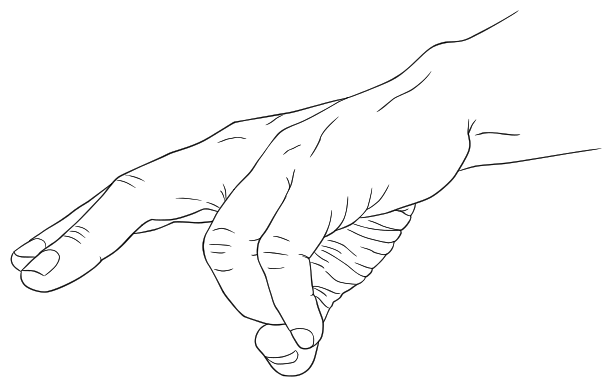
\includegraphics[width=0.69\textwidth]{../../Images/SwordFingers/SwordFingers1.pdf}
	\caption[Le sceau de l'épée]{Le sceau de l'épée}
	\label{fig:swordfingers}
\end{figure}

Le sceau a pour principal rôle de créer une spirale connectant l'extrémité du majeur gauche à la pointe de la lame et équilibrant le poids et les mouvements de l'épée.
Cette spirale est engendrée par l'extension du bras gauche dans une direction parallèle à une ligne passant par l'extrémité des deux doigts étendus.

Bien que la spirale soit aussi efficace dans les deux versions du sceau, la version traditionnelle, plus contraignante, attire beaucoup plus l'attention sur le côté gauche que ne le fait la version relâchée.

L'attention des débutants est en effet fortement focalisée sur l'épée et le côté droit, le côté gauche du corps est, le plus souvent, totalement ignoré à moins qu'ils ne soient concentrés sur le maintien strict du sceau de l'épée.
ll est donc important que les débutants n'oublient pas le sceau de l'épée en pratiquant. Ce n'est que lorsqu'ils ont acquis suffisamment d'expérience et que la spirale leur est devenue naturelle qu'ils peuvent commencer d'utiliser la forme relâchée du sceau.

\section{Manipulation}
On entend souvent répéter que l'épée doit être une extension du corps et qu'il ne faut faire qu'un avec son épée.
Ce qui peut sembler une évidence dans ce discours est toutefois loin d'aller de soi dans la pratique.
Tout d'abord, il faut considérer son épée comme un segment supplémentaire du bras, la prise de l'épée jouant le rôle d'une articulation.
Au même titre que les autres articulations, la prise doit donc être relâchée et bouger à l'unisson de tout le corps en laissant l'épée bouger librement dans la main.

En effet, si on recherche bien l'unité avec l'épée, celle-ci n'en possède pas moins sa propre individualité et une manière particulière de répondre, selon ses caractéristiques physiques, aux sollicitations du pratiquant.
Il est donc indispensable que le comportement individuel de l'épée soit pris en compte pour parvenir à harmoniser ses mouvements avec ceux du pratiquant.

Ce rapport à l'épée présente certaines similitudes avec la danse : un bon danseur en effet ne fait pas qu'imposer des pas à sa cavalière mais il est aussi capable de percevoir l'équilibre et les mouvements de celle-ci afin d'y adapter ses propres déplacements et de la conduire en douceur.
De la même manière, il ne s'agit pas d'imposer ses mouvements à l'épée mais de la guider dans la direction appropriée pour réaliser la technique souhaitée.
Les propres mouvements du pratiquant sont guidés en retour par le poids et l'élan de l'épée : si l'épée est bien une extension du corps, il n'en est pas moins vrai que le corps est lui même une extension de l'épée...
Il y a entre l'épée et le pratiquant un constant va-et-vient qui est des plus apparents dans la forme mais n'en est pas moins important en assaut libre.
De la sorte, même une épée plutôt lourde peut être manipulée efficacement et avec légèreté en utilisant le strict minimum de force musculaire, l'élan de chaque mouvement étant récupéré et réutilisé pour générer le mouvement suivant.

Le poids et l'inertie de l'épée elle même, combinés à la juste impulsion au moment opportun, apportent l'énergie nécessaire à la réalisation des techniques.
Grâce à l'inertie, le centre de gravité, emporté par l'élan de l'épée, joue le rôle d'un point d'appui permettant d'accélérer la pointe ou de la diriger vers une autre direction.
En assaut libre, les pressions exercées volontairement ou non sur la lame par l'adversaire peuvent aussi être absorbées, assimilées et transformée pour générer attaques ou ripostes.

Pour faire court, nous conclurons en disant que l'énergie est enracinée dans la fusée, qu'elle est contrôlée par le centre de l'épée et qu'elle s'exprime dans la lame.
% !TeX spellcheck = en_GB
\chapter{The \Jiben{} \Jianfa{}}\label{ch:jianfa}

The term \Jiben{} \Jianfa{} (\begin{CJK*}{UTF8}{bsmi}基本劍法\end{CJK*}) denotes what is generally referred to as the sword basic techniques or basic cuts.
It may be translated literally as: the \textit{basic}, \textit{elementary}, \textit{fundamental} (\Jiben{}) \textit{methods} (\Fa{}), of the \textit{straight sword} (\Jian{}).

The different styles of \Taijijian{} report a variable number of \Jiben{} \Jianfa{}, usually ranging from four to thirteen or more. The names of several of them are mentioned already in the \JianJing{}, a sword treatise written by \YuDayou{} around 1560, or in the \WubeiZhi{}, a military encyclopaedia presumably published in 1620.
It is not clear though whether these terms were already referring to the very same techniques as they do today in \Taijijian{}, and even more so as the \Jiben{} \Jianfa{} names are not always consistent across styles.

The \Yangjia{} \Michuan{} \Taijijian{} tradition lists eight \Jiben{} \Jianfa{}, each corresponding to one of the eight sections in the \Kunlun{} sword form: \Pi{}, \Ci{}, \Liao{}, \Zha{}, \Mo{}, \Duo{}, \Tiao{}, \Hua{}.
A ninth one, \Dian{}, is also referred to, but is sometimes described as a combination of \Pi{} and \Ci{}, possibly in order to preserve the fit total number of eight pure techniques.
Whatever the reason for it, I have the feeling that this description of \Dian{} as a combination actually acknowledges that the \Jiben{} \Jianfa{} can be mixed together.
I therefore like to consider them not as techniques \textit{per se} but rather as technical principles that, blended together, make up the actual sword techniques. The so-called basic techniques would thus be simply the techniques which are representative  of the \Jiben{} \Jianfa{} constituting their main, yet not exclusive, component. 

A close look at the Chinese characters for the eight \Jianfa{} of the \Yangjia{} \Michuan{} reveals that four of them (\Pi{} \begin{CJK*}{UTF8}{bsmi}劈\end{CJK*}, \Ci{} \begin{CJK*}{UTF8}{bsmi}刺\end{CJK*}, \Duo{} \begin{CJK*}{UTF8}{bsmi}剁\end{CJK*} and \Hua{} \begin{CJK*}{UTF8}{bsmi}劃\end{CJK*}) contain the graphic key for the knife, whereas the others (\Liao{} \begin{CJK*}{UTF8}{bsmi}撩\end{CJK*}, \Zha{} \begin{CJK*}{UTF8}{bsmi}扎\end{CJK*}, \Mo{} \begin{CJK*}{UTF8}{bsmi}抹\end{CJK*}, \Tiao{} \begin{CJK*}{UTF8}{bsmi}挑\end{CJK*}) contain the key for the hand. We may thus argue that the first four focus on how the blade is actually used for cutting or thrusting while the others rather describe the general movement (raising, whipping, etc.) independently of the weapon. As a matter of fact, the \Liao{} and \Zha{} characters can be found in the names of spear, staff or even boxing techniques mentioned in various historical martial arts manuals. The ninth technique, \Dian{} \begin{CJK*}{UTF8}{bsmi}點\end{CJK*}, whose name means \textit{pointing}, is once again an outsider: as its character does not contain the hand or the knife keys, it would exclusively refer to the point of the blade. 

The descriptions of the \Yangjia{} \Michuan{} \Taijijian{} \Jiben{} \Jianfa{} will not  be presented hereafter in their traditional order, which follows the sequence of the corresponding sections in the \Kunlun{} sword form. Instead, I will present first the four blade techniques before proceeding to the other ones. They are personal interpretations allowing for the above points of view and based upon Master Wang's teachings and historical texts. Although the contents of this chapter essentially apply to the \Yangjia{} \Michuan{} tradition, it is expected that they may none the less apply more generally, at least in part, to other styles as well. 

\fiche{
add a table describing the different energies and their scope: Pi is a way of cutting, liao defines the direction of the cut with the true edge and as such can express Pi energy...
Maybe some consideration of the sword and hand keys, correspondence between techniques
}

% !TeX spellcheck = fr_FR
\section{\Pi{}}
En chinois, \Pi{} \begin{CJK*}{UTF8}{bsmi}劈\end{CJK*} signifie \textit{couper}, \textit{fendre}, \textit{aller droit vers}. En substance, \Pi{} est une coupe fendante.

En tant que technique de base, \Pi{} est simplement décrit comme une coupe verticale descendante. Elle est souvent associée à un moulinet intérieur ou extérieur que je ne décrirai pas ici puisqu'il ne fait pas strictement partie de la technique \Pi{} et aura plutôt sa place ailleurs.

Bien que la technique formelle \Pi{} soit dirigée vers le bas, je pense personnellement que l'énergie fendante de \Pi{} peut être orientée dans toute direction. Ainsi, même des coupes horizontales ou montantes qui fendent la cible de manière caractéristique sans aucun mouvement de trancher peuvent être en quelque sorte considérées comme affiliées à cette énergie.

La technique emblématique formelle \Pi{} se prépare en levant la poignée de l'épée à hauteur d'oreille pendant que l'on s'assied dans la jambe opposée à la main armée. La prise doit être relâchée mais fermement maintenue entre le majeur, l'annulaire et le pouce. Le contact relâché des autres doigts maintient un contrôle de la poignée tout en permettant une certaine flexibilité de la prise.
Dans un contexte moins formel et moins statique, on peut combiner cette préparation à un déplacement pendant une parade ou une esquive, dans une transformation continue de l'action défensive en riposte.

Dans la première phase de la coupe, la main est envoyée en diagonale et tire l'épée en avant vers le bas dans la direction du pommeau pour accélérer la lame. La force de biais exercée par la main sur la poignée entraîne ainsi graduellement la rotation de l'épée autour de son centre de gravité (fig. \ref{fig:pi_cut} a).

Ce mouvement tire son énergie de l'expansion du corps et le cas échéant d'un pas vers l'avant pour une portée plus importante et un gain de puissance.

Ensuite, dès que le centre de gravité a passé en avant de la main (fig. \ref{fig:pi_cut} b), celle-ci cesse d'exercer toute action et ne fait plus que suivre la poignée en maintenant simplement un contrôle relâché mais ferme de la trajectoire de l'épée. La lame se déplace ainsi librement avec une trajectoire non perturbée au moment où elle atteint la cible et toute l'énergie cinétique accumulée lors de la phase d'accélération est alors transférée dans la coupe (fig. \ref{fig:pi_cut} c).

\begin{figure}[ht]
\centering
	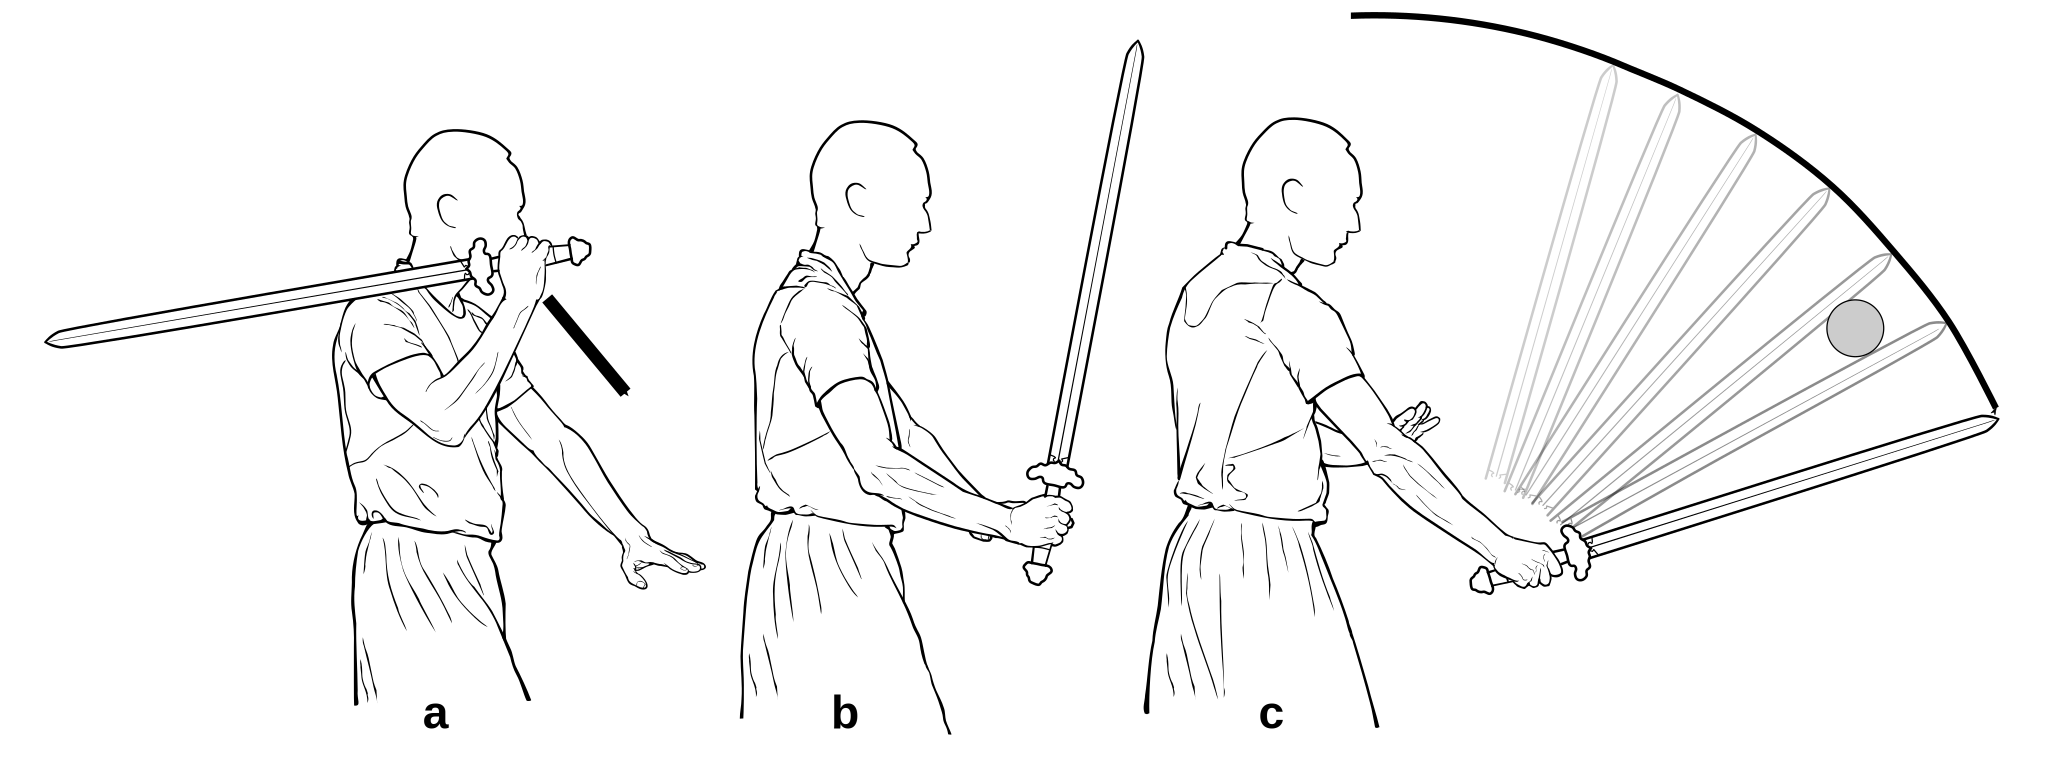
\includegraphics[width=1.00\textwidth]{../../Images/JibenJianfa/Pi/Pi_juxtaposed.pdf}
	\caption[Coupe \Pi{}]{Coupe \Pi{} : (a) Partant d'une position haute de l'épée, la main droite la tire vers le bas pour accélérer la lame; (b) montre la fin de la phase d'accélération, à partir de cet instant, la main n'exercera plus d'action sur la poignée; (c) la main suit la poignée avec juste un contrôle ferme de la trajectoire de l'épée de manière à ce que la lame puisse librement traverser la cible représentée par un cercle gris. Notez que la trajectoire de la pointe n'est pas un cercle mais un arc allongé.}
	\label{fig:pi_cut}
\end{figure}

Il est absolument indispensable que le plat de la lame soit parfaitement aligné avec la trajectoire de la l'épée pour garantir que le poids de la lame soit derrière le tranchant pour le pousser à travers la cible. Si jamais la lame atteignait la cible avec un angle, aussi petit soit-il, elle tendrait à tourner autour de son axe et pourrait rebondir dangereusement au lieu de trancher. Lorsque l'alignement est correct, au contraire, et que la prise est relâchée, la lame pourra traverser la cible de part en part sans retour notable.

Après la coupe, la poignée bute naturellement contre le talon de la main et les doigts resserrent leur prise pour arrêter l'épée dans une position de garde à hauteur de taille, sans aucune tension ni rebond. Grâce à une bonne structure corporelle, l'énergie de l'épée retourne ainsi au corps, aidant le recentrage, et la préparation de la technique suivante.
% !TeX spellcheck = fr_FR
\section{\Hua}
Le verbe \Hua{} \begin{CJK*}{UTF8}{bsmi}劃\end{CJK*} signifie \textit{délimiter}, \textit{tracer}. Ce caractère est aussi une variante du mot désignant un trait dans un caractère chinois.
La partie de gauche de ce caractère étant la clé du pinceau, ces observation suggèrent que cette technique évoque la notion de calligraphie, d'écriture et de dessin.

Le \Yangjia{} \Michuan{} présente la technique \Hua{} emblématique comme une coupe horizontale ou un large mouvement horizontal dans le but de maintenir les adversaires à distance. L'idée est ici de balayer l'espace avec l'épée pour délimiter la zone la plus large possible autour de soi et d'entailler quiconque ose s'approcher.

D'une manière plus générale, les coupes \Hua{} ne sont pas systématiquement horizontales et s'appliquent à différentes distances, depuis des entailles réalisées à longue distance avec la pointe de l'épée, jusqu'à des coupes glissées avec toute la longueur du tranchant à courte distance. Dans tous les cas, les coupes \Hua{} ont pour caractéristique commune le fait que la lame trace progressivement une longue entaille, au contraire de \Pi{} qui fend la cible d'un coup. 

Pour réaliser une coupe \Hua{} à longue distance, l'épée est lancée en avant et, lorsque le bras a presque atteint son extension complète, juste avant que la lame ne frappe la cible, la prise se resserre doucement sur la poignée pour assurer la connexion entre les centres de l'épée et du corps. La rotation continue ainsi à partir de l'épaule tandis que l'épée tire le corps en avant jusqu'à ce que la portée maximale soit atteinte (fig. \ref{fig:hua_cut} a-c). Ensuite, la prise agissant comme un levier, l'inertie de l'épée repousse la poignée contre le talon de la main, engendrant un mouvement vers l'arrière qui génère une coupe glissée et recentre le corps dans une posture de garde (fig. \ref{fig:hua_cut} d-f). 

\begin{figure}[ht]
\centering
	\includegraphics[width=1.00\textwidth]{../../Images/JibenJianfa/Hua/Hua.pdf}
	\caption[Coupe \Hua{}]{Coupe \Hua{} : (a) \'{A} partir d'une position haute de l'épée, (b) la main droite lance le pommeau vers l'avant; (c) montre la fin de la phase active de la technique; (d) à (f) pendant la phase passive, l'inertie de l'épée repousse la main en arrière, réalisant la coupe glissée et recentrant le corps en position.}
	\label{fig:hua_cut}
\end{figure}

\'{A} plus courte distance, la dynamique des coupes \Hua{} utilise moins l'inertie de l'épée mais s'appuie plus sur la structure et le mouvement du corps. Dès que le tranchant est en contact, la coupe est effectuée en pressant le tranchant contre la cible et en tirant l'épée selon une direction parallèle à l'épée, en se déplaçant ou en tournant le corps. Il est parfois possible, en particulier en passant dans le dos de l'adversaire, de réaliser avec le faux tranchant une coupe \Hua{} à courte distance.

En plus d'être une coupe glissée, \Hua{} peut aussi être utilisé pour maintenir des adversaires à distance ou les obliger à réagir de façon à exploiter leur action et prendre le contrôle du rythme. Pour ce faire, on peut lancer une coupe \Hua{} sans toutefois s'engager totalement, ou faire des moulinets tout en avançant. La distance doit dans ce cas est suffisamment courte pour que ces coupes soient clairement perçues comme une menace bien qu'on puisse être légèrement hors de mesure. La distance idéale est à la limite supérieure de la mesure courte, distance à laquelle, bien qu'elle soit incertaine, une touche est tout à fait plausible et l'adversaire ne peut que se sentir obligé de réagir défensivement. Il est important dans ce cas de se préparer à doubler avec une attaque plus engagée ou un contrôle de la lame selon les circonstances. C'est cette seconde intention qui permettra de prendre l'initiative en exploitant l'action de l'adversaire.

En rompant la distance après une attaque infructueuse, il est possible de maintenir l'adversaire à distance avec une série de moulinets que Maître Wang Yennien décrivait également comme étant des coupes \Hua{}. Cette application de la technique correspond parfaitement à la traduction \textit{délimiter} puisqu'elle crée en effet une zone de sécurité empêchant l'adversaire d'entrer et d'attaquer pendant qu'on se place hors de mesure.

% !TeX spellcheck = fr_FR
\section{\Ci{}}
On trouve le mot \Ci{} \begin{CJK*}{UTF8}{bsmi}刺\end{CJK*}, signifiant \textit{estoquer}, \textit{percer}, \textit{poignarder}, dans le \WubeiZhi{} comme terme générique désignant l'ensemble des techniques d'estoc à l'épée. D'autres traités anciens le mentionnent aussi pour décrire les estocs avec diverses armes. 

Dans la tradition du \Yangjia{} \Michuan{}, \Ci{} est défini comme un estoc horizontal ou remontant, poussant la pointe puissamment à travers la cible. 

On réalise généralement la technique formelle en commençant sur le pied droit, pied gauche en avant, soit avec une passe avant (\Ci{} long), soit avec un simple transfert de poids sur le pied gauche (\Ci{} court). Dans le contexte formel des exercices et de la forme, la cible du \Ci{} court est l'abdomen, celle du long est la base de la gorge. En assaut par contre, on peut viser d'autres cibles telles que le torse, ou même le visage.

Que la technique réalisée soit longue ou courte, on commence invariablement par créer dans le corps une structure spiralée connectant le pied gauche et l'épée. Dès que la taille bouge, le bras droit pousse sur la poignée et se lève en un mouvement spiralé qui s'achèvera avec une position d'épée horizontale, sur son plat, le pommeau orienté vers la hanche gauche. Dans le même temps, on transfère le poids sur le pied gauche. La prise de l'épée s'adapte progressivement pour maintenir une connexion ininterrompue entre la main et la poignée, sans aucun angle, permettant de pousser sans effort l'épée vers avant. Cet ajustement permet également d'exercer sur la poignée une action oblique atteignant au delà de la garde le point générant un point pivot dans la pointe de la lame pour la stabiliser\footnote{Voyez le chapitre \ref*{ch:epeechinoise} pour de plus amples détails sur les points pivots.}. 


La passe avant du \Ci{} long permet une portée plus longue. Le bras droit doit être étendu avant d'avancer pour augmenter la précision de l'estoc et placer le corps derrière l'épée, aussi loin que possible du danger. Engager la lame de l'adversaire pour la contrôler avec la garde ou le fort de la lame, permet encore une meilleure protection. 

\begin{figure}[ht]
\centering
	\includegraphics[width=1.00\textwidth]{../../Images/JibenJianfa/Ci/Ci_thrust_arc.pdf}
	\caption[Estoc \Ci{} long]{\`{A} la fin de l'estoc \Ci{} long, l'épée est alignée avec la hanche gauche mais sa pointe est dirigée vers le centre, visant la base de la gorge. La puissance de toute la structure du corps se concentre dans l'épée pour pousser la pointe à travers la cible.}
	\label{fig:ci_thrust}
\end{figure}

Idéalement, le talon droit devrait toucher le sol exactement au moment où la pointe de la lame atteint la cible. Le relâchement de la structure achève alors le pas en poussant la lame au travers de la cible. Il est important de ne pas se laisser tomber dans la jambe droite de manière à conserver une capacité de se retirer rapidement en cas de nécessité. Cela ne signifie toutefois pas qu'on ne doit jamais transférer le poids sur la jambe droite, mais que la polarité vide/plein entre les deux jambes doit être maintenue en toutes circonstances pour éviter la double lourdeur. L'arc de force venant du pied gauche, traversant le dos, spiralant le long du bras droit jusqu'à la pointe de l'épée, et soutenu par la spirale du bras gauche, génère ainsi une structure à la fois puissante et mobile.

% !TeX spellcheck = en_GB
\section{\Duo}
The translation of \Duo{} \begin{CJK*}{UTF8}{bsmi}剁\end{CJK*}, referring to the cooking term \textit{to mince}, somehow suggests repetition and cutting using a part of the blade further away from the tip than \Pi{}. The movement itself is a combination of a forward extension with some sort of shearing, as if using a large cooking knife to mince herbs or vegetables.

In the \Yangjia{} \Michuan{} tradition, the emblematic \Duo{} is performed with both arms extended almost in line with the sword's blade (fig. \ref{fig:duo_full}). 


\begin{figure}[ht]
	\centering
	
	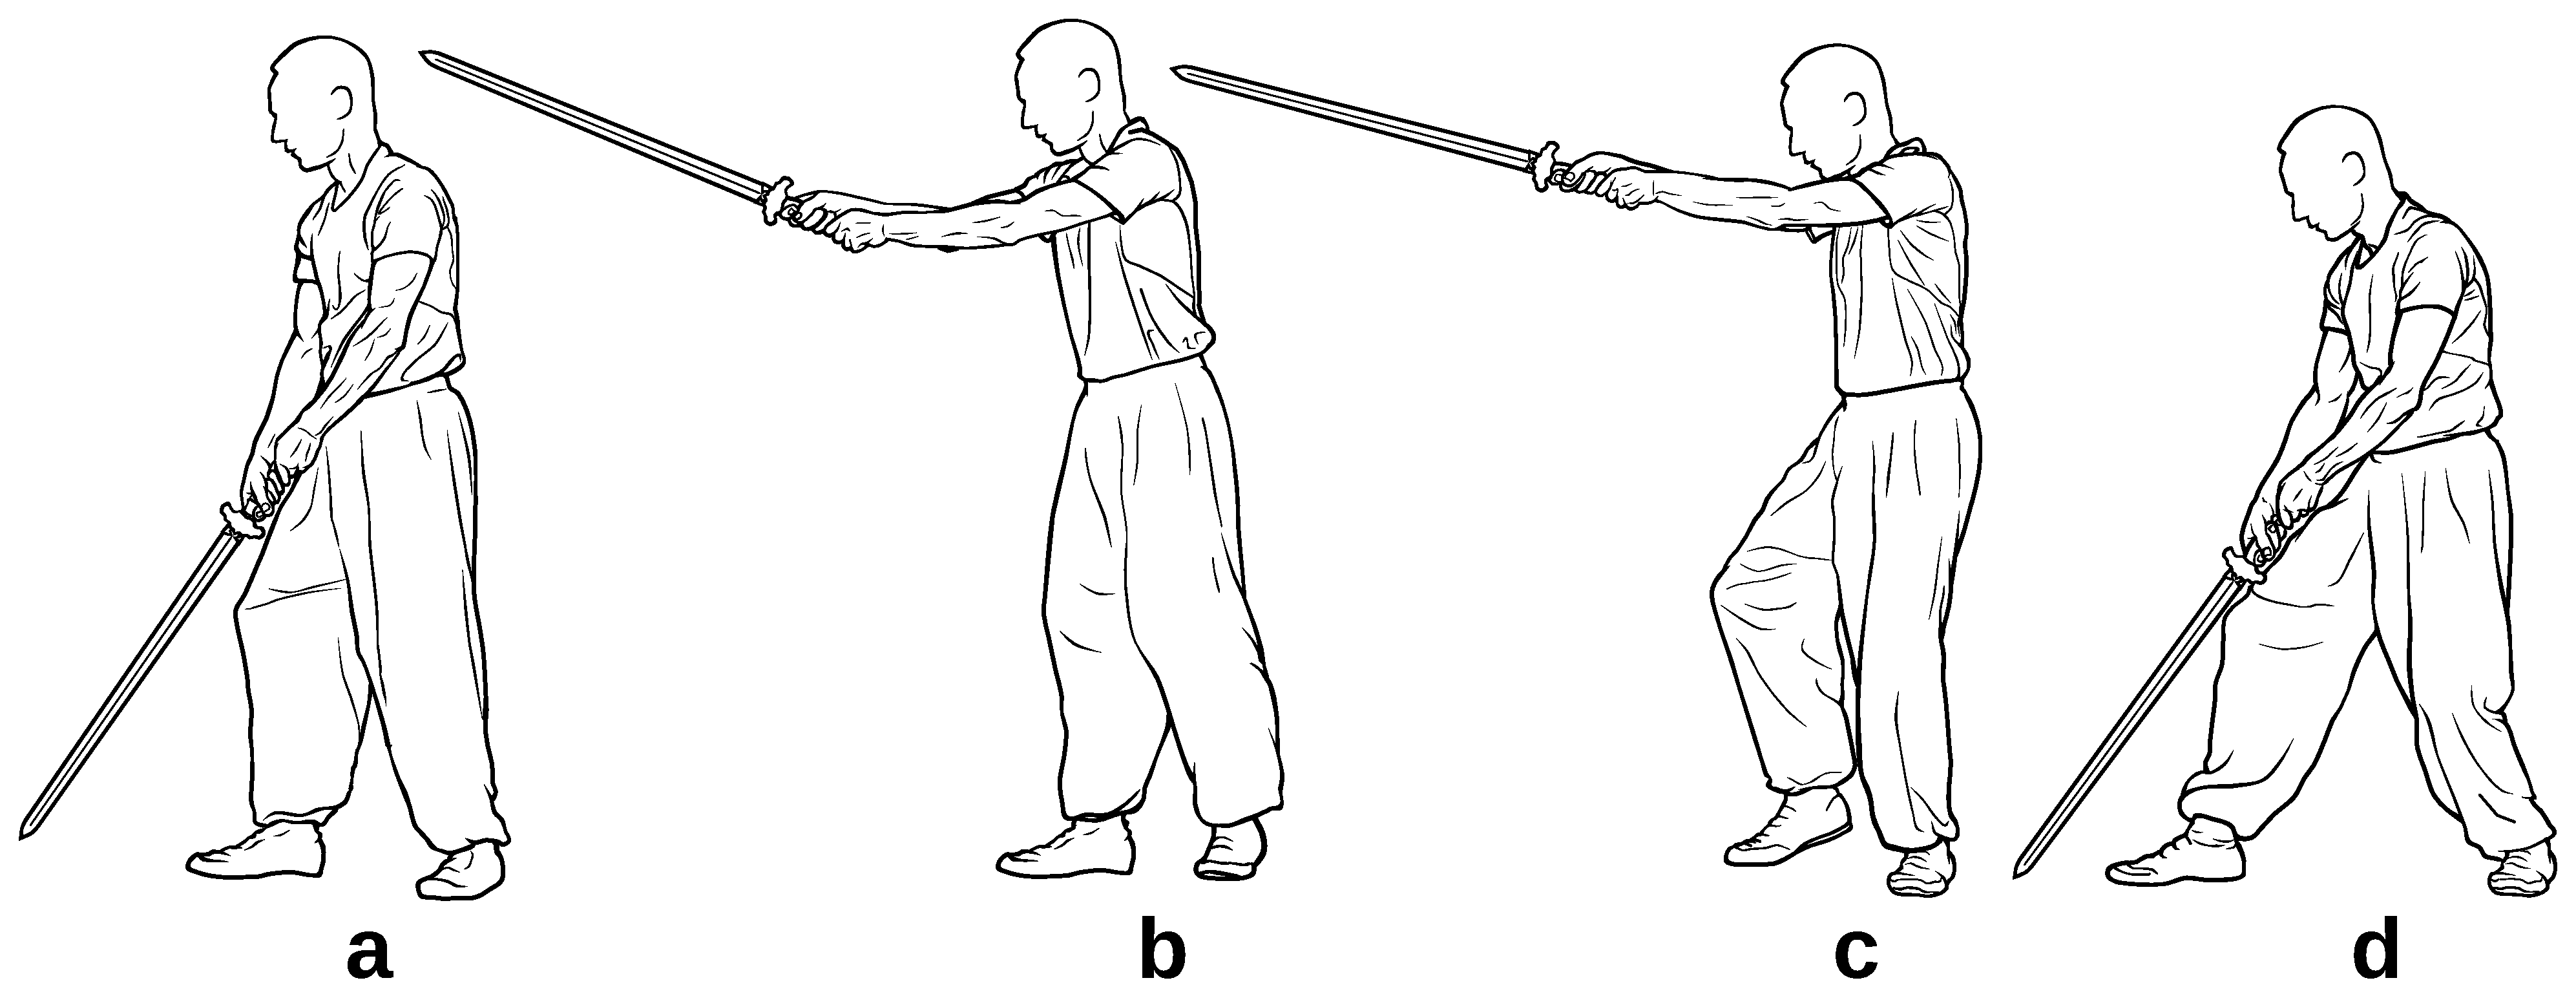
\includegraphics[width=1.00\textwidth]{../../Images/JibenJianfa/Duo/Duo.pdf}
	\caption[Advancing \Duo{}]{\Duo{} in the forward direction. From a low guard (a), raise the sword with a transfer of the weight onto the right foot (b), invert polarity and transfer the weight back onto the left foot (c), drop the sword while sinking in the left leg and advancing the right foot.}
	\label{fig:duo_full}
\end{figure} 

Even though both hands are in contact with the handle,  this should not be mistaken for a true double handed grip of the sword. While raising the sword and advancing, the right hand holds the sword while the left hand provides the structure and power coming from the waist by acting on the pommel along the direction of the blade. The combination of the right hand's passive role with the left hand's action creates a polarity resulting in a movement of the sword perpendicular to the axis of the right arm. When lowering the sword, the roles of both hands are inverted (fig. \ref{fig:duo_detail}). 

\begin{figure}[ht]
	\centering
	
	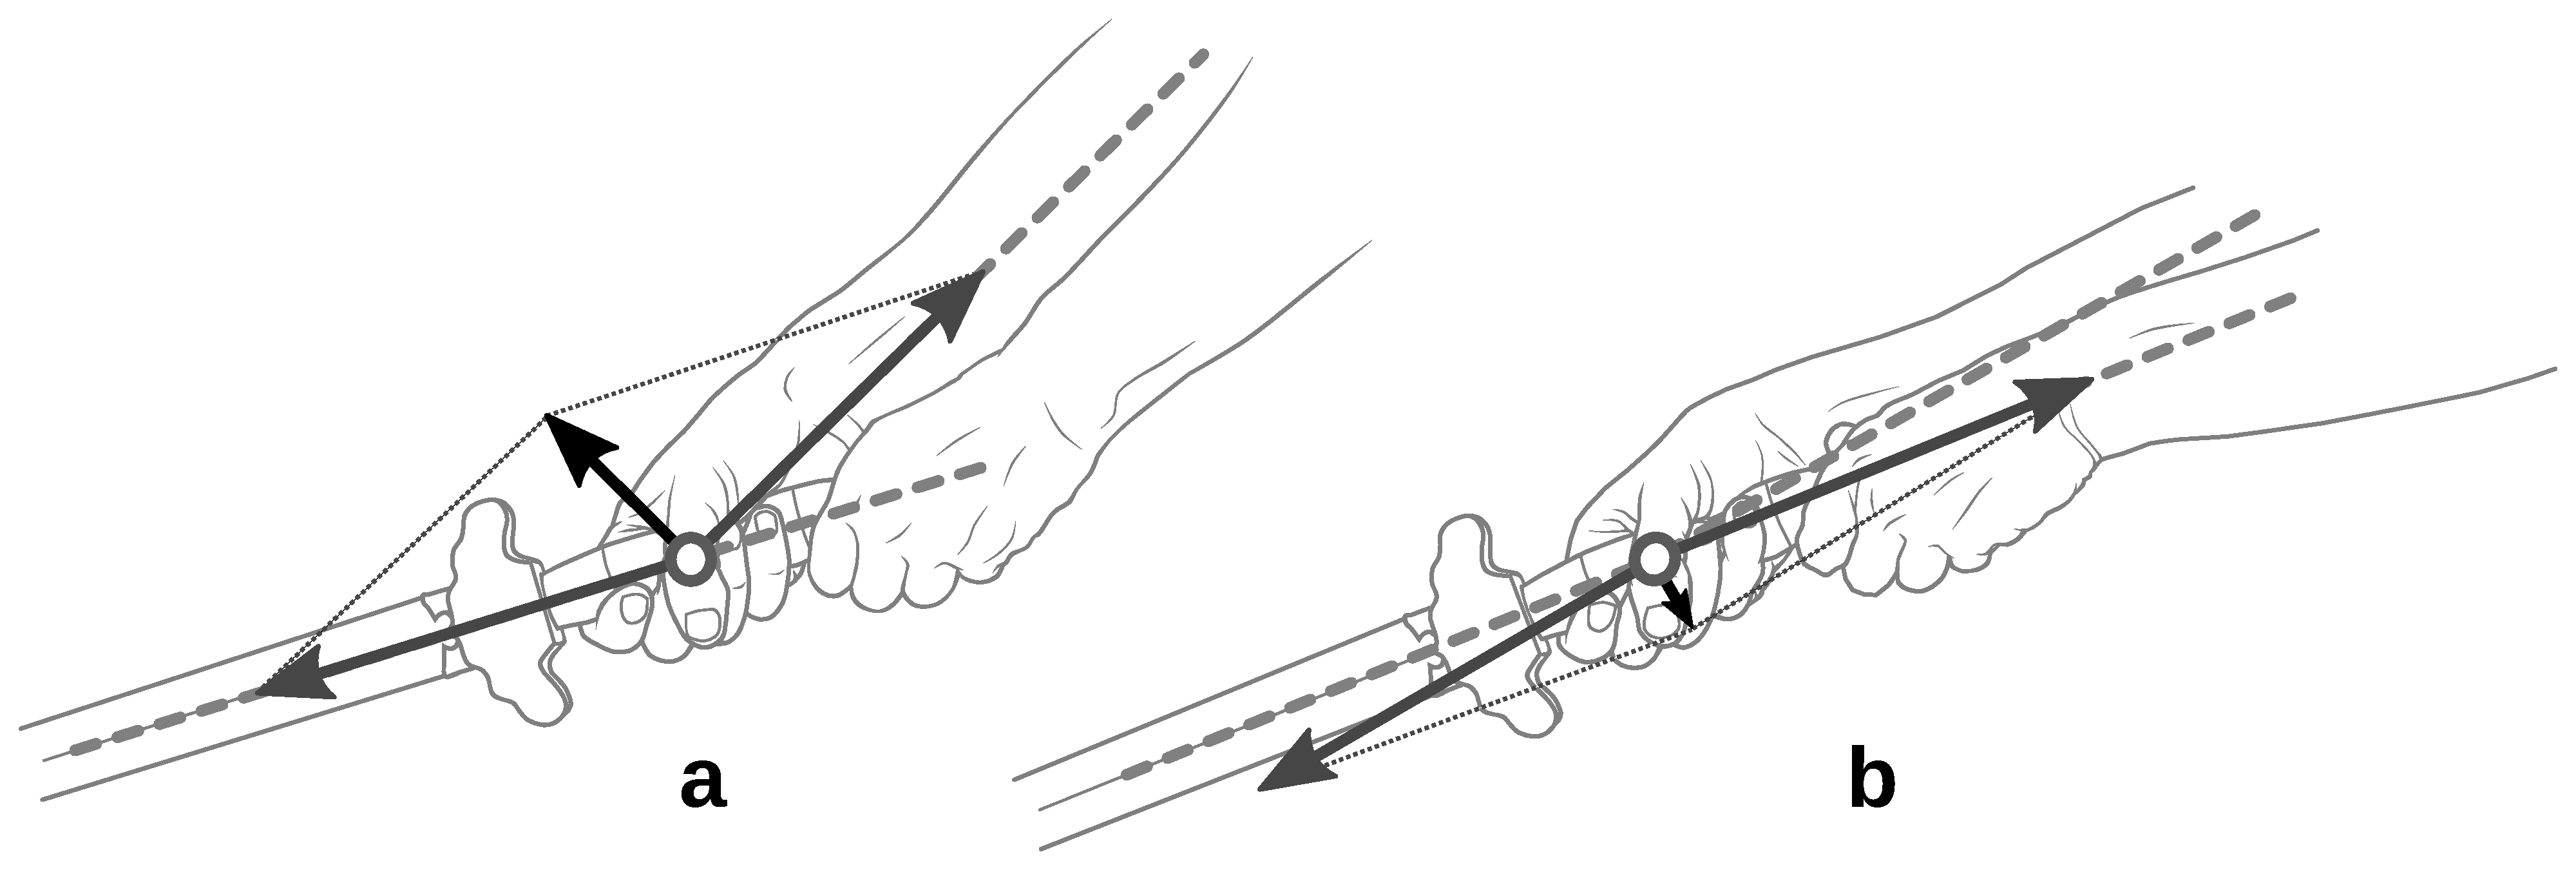
\includegraphics[width=1.00\textwidth]{../../Images/JibenJianfa/Duo/DuoDetail.pdf}
	\caption[Balance of forces in \Duo{}]{(a) To perform a forward rising \Duo{}, the left hand pushes the handle in the direction of the blade tip while the right arm passively balances the pushing force. Due to the angle between the pushing direction and the right arm, the resulting force perpendicular to the right arm pushes the sword upwards.\\
	(b) To perform a forward descending \Duo{}, the right hand pushes the handle while the left arm passively balances this force. The resulting force perpendicular to the left arm, draws the sword downwards.
	}
	\label{fig:duo_detail}
\end{figure} 

The power of the ascending forward \Duo{} thus originates in the weight transfer from the rear leg onto the fore leg, is transmitted to the sword by the left/rear hand with the right/fore hand exactly and passively balancing the forces to effortlessly generate the technique. An effective connexion between the waist and the sword will allow the explosive expression of the \Duo{} technique. 
This method somehow echoes the precepts found in the \JianJing{} stating that, when wielding a double-handed sword, power is first in the waist, then in the rear hand, and finally in the fore hand.

For the retreating \Duo{}, however, the hands play a reversed role: the right hand is active when raising the sword, and passive otherwise. As a rule of thumb, advancing or retreating, the active hand is always the one on the same side as the foot that is moving.

Since, when cooking, herbs are usually minced by cutting downwards, we may argue that the active phase of \Duo{} is the descending one. However, if we examine attentively the actual movement of a kitchen knife when mincing, we may discover that its form when cutting actually corresponds to the rising phase of \Duo{}. The main difference is that the tip of the knife stays down in contact with the table whereas the point of the sword rises up. But, in both cases, the edge follows the same movement relative to the tip. 
However, it is perfectly possible to be active in both phases, the actual passive phase being the transition movement between the ascending and descending parts of the technique. Thus, \Duo{} can be a raising thrust or cut as well as a descending cut, or, combined with \Mo{} energy, an action on the opponent's blade, either ascending to intercept and deflect or descending to shear. 

It is worth noting at this point that, since both hands are in contact with the hilt, the sword is always in line with the axis of the body. This axis is more to the left when we are on our left foot, in the low on-guard position that precedes the ascending forward phase of \Duo{}. Then, during the lifting phase of the movement, the axis is shifting to the right before being transferred back to the left when descending. Therefore, in the deflect/shear application of  \Duo{} in combination with \Mo{}, during the upward interception/deflection, transferring the weight onto the right/forward leg gently pushes the opponent's tip away, allowing the descending shear to naturally aim at the centre of the opponent's sword, deflecting it further to open the way for a hit while preventing any counter attack. 

\fiche{The simplest application of \Duo{} starts with a lower guard as an invitation for the opponent to prepare an attack. We can then engage and deflect with a \Duo{} before placing our riposte or we may take advantage of the explosive nature of the movement and use an offensive \Duo{} to thrust directly during the opponent's preparation.
\Duo{} is often performed in series of two to three movements, not more to avoid predictability, as seen for the double-handed version in the \Kunlun{} form. We can usually identify three periods in these series: The first \Duo{} movement would intercept an incoming attack, either a \Pi{} or a \Hua{} cut from above or a high level \Ci{} thrust.Then, the second one will deflect the opponent's blade to open the way for the third \Duo{} thrust. Of course, this is not a fixed pattern, and the first movement can be followed by any appropriate technique depending on the circumstances. For instance, instead of deflecting, the second step may accompany the opponent's blade to control it while entering to prepare the riposte.}

Although the classic movement is done with two hands, it is also possible to perform a \Duo{} with one hand only. In this case, the heel of the hand plays the same role as the rear hand in the two-handed version while the first three fingers \textemdash{} the index and middle fingers, and the thumb \textemdash{} play the part of the forehand (figure). 

During the ascending phase, the handle of the sword is pushed forwards by the heel of the hand and simultaneously pulled by the first three fingers. Given a good structure in the on-guard position, it is then possible, even with only one hand, to swiftly and effortlessly raise the sword from a low to a high position, for thrusting or engaging.  
\fiche{When descending, the fore fingers relax their grip while the ring and little fingers are tightened to pull the handle. Some intention should be put at the base of the index to gently push the handle downwards in the forward direction. The resulting structure allows to capture and deflect the centre of the opponent's sword by shearing or to perform a powerful cut while retreating.}
The alignment of the sword is quite similar to the two-handed version, with the tip of the blade in line with the body axis. However, the structure is not as strong as in the two-handed \Duo{} and, as a result, the shearing actions are not as powerful. However, this version of the movement is useful for quickly engaging the opponent's blade or a sudden attack from a lower guard. 

\fiche{
These actions can be chained, as in the \Kunlun{} sword form, by two or three, first intercepting the opponent's blade before deflecting and hitting with a double or treble shearing. 
the polarity between the hands allows the crossed links between hand and foot. 
}
% !TeX spellcheck = fr_FR
\section{\Liao}
\Liao{} \begin{CJK*}{UTF8}{bsmi}撩\end{CJK*} est une coupe montante.
% !TeX spellcheck = en_GB
\section{\Zha}
\Zha{} \begin{CJK*}{UTF8}{bsmi}扎\end{CJK*} is a downward thrust.
\fiche{
	spiralling arc on the outside, from the foot to the point, passing through the back and the outside of the arm and along the true edge. The back is stretched and the breast is relaxed. There is a connection between the foot and the point. The weight of the body and the rotation of the waist inwards will generate the thrust. The arm extends in coordination but not excessively
	The unarmed hand can control the opponent's arm, especially when chained after parrying \Liao{}.
	
	check the translation and make sure to use the simplified character
	translation: set up (a tent)
	
	rem: there exists another character which is simplified into this one and is pronounced at the first tone and means
}
% !TeX spellcheck = en_GB
\section{\Mo}
\Mo{} \begin{CJK*}{UTF8}{bsmi}抹\end{CJK*} encompasses all the techniques that take control of the centre of the opponent's blade.
\fiche{
	principle of controlling, deflecting, directing, listening
	the intention is located closer to the forte
	
	translation: put, spread (butter, etc.), wipe
	use the simple character
	
	maybe related to a variety of techniques used to parry, such as wash, shave, shear. ..
	
	radical mo is probably phonetical although it means powder (waste, residuals)
	
	sliding contact of the blades (wipe) with a deflecting action of control thanks to the opposition of the forte against the feeble of the opponent,  this is found in blade capture (coulé, opposition, ...) or the control of the blade during attacks
	
	lateral and aiming at the centre of the opponent's blade, if only lateral we give way to transformation by the opponent and we don't have control of their blade. 
	
	relationship with feeling through the blade and cover
	during parries, absorption, deflection, protection
}

% !TeX spellcheck = fr_FR
\section{\Tiao}
\Tiao{} \begin{CJK*}{UTF8}{bsmi}挑\end{CJK*} est une coupe rapide réalisée avec le faux tranchant.

% !TeX spellcheck = fr_FR
\section{\Dian}
\Dian{} \begin{CJK*}{UTF8}{bsmi}點\end{CJK*} est un estoc rapide ou une coupe légère réalisée avec l'extrémité de la lame.

\fiche{
\section{What makes a cut effective? }
relaxation, blade alignment
distance
must travel through the target
split or slice

\section{ What makes a thrust effective?}
point control, see pivot points in chapter 2
distance
no need for more than a few centimetres in the target to reach a vital organ
}

% !TeX spellcheck = fr_FR
\chapter{Les déplacements}\label{ch:deplacements}

Ce chapitre discutera des déplacements et systèmes de pas dans le \Taijijian{}.
\part{Escrime du \Taijijian{}}
% !TeX spellcheck = fr_FR
\chapter{La distance et le temps}\label{ch:distancetemps}

De même que pour tout art martial, le temps et la distance sont des notions essentielles en escrime.
Ce n'est que par leur maîtrise que l'on peut vraiment espérer devenir une fine lame.

Intimement imbriqués, ces deux concepts ne sont toutefois pas des notions absolues et fixes ni des dimensions physiques réelles.
Tout en étant d'une aide incontestable pour décrire et commenter objectivement les actions d'escrime, ils recouvrent le sens du temps et de la distance dans un contexte de confrontation, c'est-à-dire la perception que peuvent avoir les adversaires de leurs capacités d'action relatives.
En tant que tels, le temps et la distance sont au c\oe{}ur des tactiques et de la stratégie de l'escrime.

\section{Temps d'escrime} \index{temps d'escrime}
Le \emph{temps d'escrime} est une unité de temps définie comme la durée d'une action simple : un pas, une coupe, un estoc, une parade, etc. \index{actions simples}
Le nombre d'unités de temps que dure une action combinée est le nombre d'actions simples consécutives qui la composent, des actions simples simultanées ne comptant que pour une unité de temps.
Par exemple, deux temps sont nécessaires pour parer en passant puis riposter.

Le temps d'escrime ne correspond pas strictement au temps d'horloge, il ne s'agit pas d'une durée définie puisqu'une action simple durera plus ou moins longtemps selon la vitesse à laquelle elle est exécutée.
Le temps d'escrime est plutôt lié à la notion d'engagement dans une action sous-tendue par une intention. \index{intention} 
Tant que le bretteur ne s'est pas totalement engagé dans son action, il peut transformer \index{transformation} et modifier son intention durant la même unité de temps.
Ce n'est qu'après engagement total qu'il devient impossible d'interrompre le cours de l'action et de changer d'intention pendant le même temps d'escrime.
Ceci ne signifie toutefois pas qu'une action doit être nécessairement menée à son terme dès qu'elle a été engagée mais seulement que les transformations prennent plus de temps lorsque l'intention est totalement exprimée.

Cette notion tactique primordiale est utilisée dans les feintes et fausses attaques.
Comme nous le verrons plus loin, lors d'une feinte, on ne s'engage pas totalement dans l'action offensive mais celle-ci doit être suffisamment convaincante pour forcer l'adversaire à s'impliquer totalement dans la parade de ce qu'il croit être une attaque. 
Il est alors possible de modifier l'action initiale dans le même temps et lancer la véritable attaque alors que l'adversaire est tout occupé à sa réaction initiale.
En règle générale, il est préférable d'éviter de s'engager trop tôt dans une action de manière à préserver aussi longtemps que possible la capacité de transformer et de s'adapter efficacement aux réactions de l'adversaire.

Le temps d'escrime est donc une notion théorique permettant d'évaluer la capacité d'initiative, de transformation ou de réponse des bretteurs durant les différentes actions.
On peut ainsi formaliser le cours des actions simples pendant l'étude d'une \emph{phrase d'arme}, quelle que soit la vitesse à laquelle elle est réalisée et en supposant que les deux adversaires sont aussi rapides l'un que l'autre.
Bien entendu, en réalité, certains escrimeurs sont plus rapides que d'autres mais en vérité, la vitesse n'a aucune importance. Seul le tempo compte vraiment : l'action juste au bon moment.  
Il est toujours possible de compenser une moindre vitesse par la mise en \oe{}uvre efficace de techniques et tactiques et, par-dessus tout, par la maîtrise du rythme.\index{rythme}
Un bretteur plus rapide peut perdre son avantage s'il est forcé par un adversaire plus compétent d'utiliser plus de temps d'escrime pour ses actions. 
Cette stratégie est parfois utilisée par certains escrimeurs qui, tout en prenant leur temps, n'ont de cesse de maintenir leur adversaire dans une situation d'urgence permanente.
Qu'ils le fassent en maintenant leur adversaire sous la menace constante d'une touche ou en sortant systématiquement de ses lignes d'attaque, ils imposent leur rythme et ne laissent pas leur adversaire reprendre l'initiative.
Pour atteindre ce but, il leur est toutefois indispensable de rester connecté à leur adversaire et que leurs mouvements et les menaces qu'ils lui font soient parfaitement adaptées à ses réactions.
En d'autres termes, le rythme du combat est en réalité une combinaison des rythmes des deux adversaires.
Bien que le rythme d'un escrimeur puisse dominer celui de l'autre, il y a toujours interdépendance : il est essentiel d'être connectés et reliés en permanence.

La capacité à comprendre et suivre le rythme de l'adversaire tout en dissimulant le sien propre est donc fondamentale pour pouvoir saisir l'instant juste et prendre l'avantage.
Il est essentiel de rester en permanence à l'écoute des mouvements de l'adversaire et de ne pas se laisser entraîner dans une anticipation inconsidérée par une régularité trompeuse du rythme.
Une attention toute particulière devrait également être portée à ne pas adopter un rythme trop régulier qui serait par conséquent facilement prévisible par l'adversaire.
Contrôler le rythme implique un état d'esprit relâché nous assurant d'être constamment prêt à nous adapter à la situation et à la transformer à notre avantage en répondant aux actions de l'adversaire de manière imprévisible.
Cependant, bien plus que d'avoir des réactions rapides  \textemdash{} vitesse n'est pas précipitation \textemdash{} il s'agit assurément de se tenir sur le fil d'un perpétuel présent, lâchant le passé et accueillant le futur sans s'attacher à aucune technique préconçue.

\section{Distance et mesure}\index{distance}
De même que le temps d'escrime ne représente pas une durée objective, l'effet de la distance entre les deux adversaires sur leur capacité relative à s'atteindre mutuellement est ici plus importante que leur distance physique réelle.
On définit ainsi la mesure \index{mesure} comme la distance en deçà de laquelle il est possible d'atteindre l'adversaire en un temps d'escrime.
En d'autres termes, c'est une distance suffisamment courte pour ne pas nécessiter plus d'un pas pour toucher.
Si au moins deux pas sont nécessaires, on est dit hors mesure.

On peut, à partir de là, définir trois distances en mesure :
\begin{enumerate}
\item \emph{Distance de garde} ou \emph{mesure longue} : 
un pas est nécessaire pour toucher. Cette distance offrant un bon compromis entre une attitude prudente et une tendance plus agressive, c'est une distance fréquemment adoptée pendant un assaut libre.
\item \emph{Distance de touche} ou \emph{mesure courte} : 
à cette distance, il est possible de frapper avec la partie appropriée de la lame sans avoir à faire un pas ni vers l'avant ni vers l'arrière.
\item \emph{Distance rapprochée}: 
cette distance est trop courte pour permettre une utilisation efficace de la lame, seules les techniques de corps à corps sont utilisables : coups de pied, de poing, saisies, etc. 
\end{enumerate}

Mais la mesure est plus qu'une distance.
Elle est influencée en effet par les postures des escrimeurs et leurs angles d'attaque respectifs.
La garde et la position des pieds détermine la portée maximale de l'épée atteignable en un temps d'escrime par une action simple : pas, transfert de poids, rotation du bras et du corps.\index{actions simples}
L'angle d'attaque et la manière dont l'adversaire se couvre sont les facteurs principaux déterminant si la cible pourra alors être atteinte par une coupe ou un estoc efficace.

Il faut garder à l'esprit que l'angle d'attaque comme la portée de l'épée ne doivent pas être uniquement considérés dans le plan horizontal mais en trois dimensions.
Ainsi, en toute situation, les cibles les plus proches sont celles approximativement situées à hauteur d'épaule, c'est-à-dire, la plupart du temps, le haut de la poitrine et la gorge.
Il est possible d'atteindre les cibles plus basses en avançant, mais aussi en s'accroupissant ou en se penchant de manière à abaisser l'épaule en face de la cible.

La figure \ref{fig:distance_stance} montre l'effet de la posture, des déplacements et de la hauteur de la cible sur la portée de l'épée.

\begin{figure}[ht]
\centering
	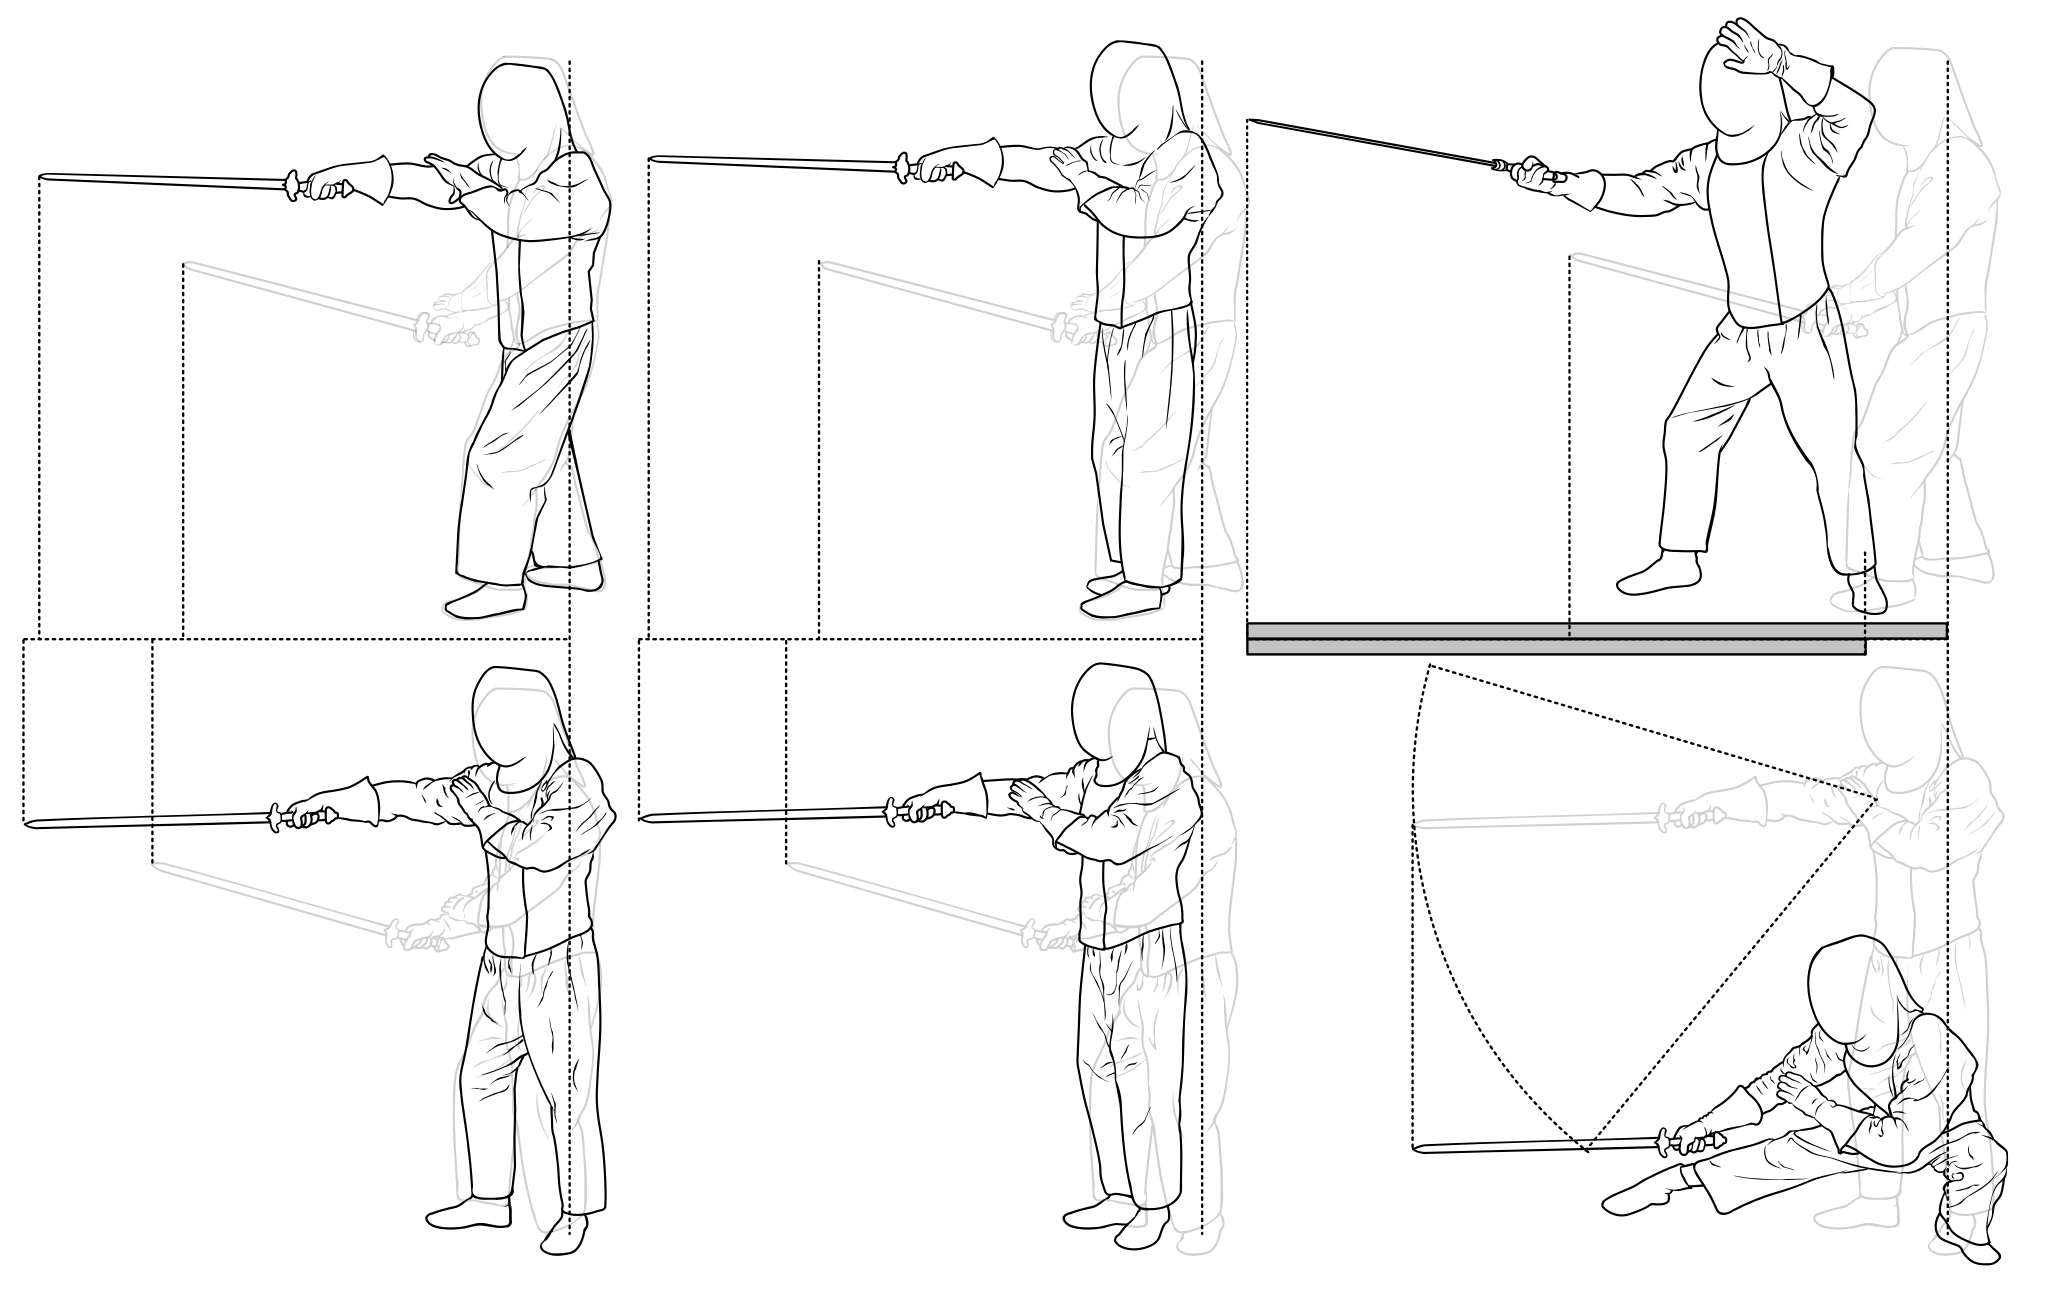
\includegraphics[width=1.0\textwidth]{../../Images/DistanceTime/distance_stance.pdf}
	\caption[Posture et mesure]{Quelques exemples de postures et leur portée en estoc.\\
	La colonne de gauche montre la distance atteinte par l'extension du bras à partir de la position de garde initiale (représentée en gris). Cette distance est légèrement plus longue avec le pied droit en avant (figure du bas) grâce à la plus grande amplitude de rotation du corps poussant l'épée plus en avant. On peut faire une observation similaire sur la position de garde qui s'étend légèrement plus en avant avec le pied droit devant. La même remarque s'applique à la colonne du milieu montrant la distance atteinte en étendant le bras et en serrant le pas. La différence est toutefois moindre ici en raison d'une distance plus courte entre les pieds.\\
	La figure en haut à droite montre la portée maximale d'un estoc. Ainsi, le rectangle gris supérieur représente la longueur de la mesure en partant le pied gauche en avant. Grâce au déplacement de l'axe sur le pied gauche et à la passe avant, cette mesure est plus longue qu'en partant directement avec le pied droit devant.\\
	Sur la figure en bas à droite, l'arc de cercle représente la portée verticale de l'épée en se tenant debout sans faire de pas. Bien qu'elles puissent ne pas être horizontalement plus loin de l'axe du corps, les cibles basses n'en sont pas moins hors d'atteinte à moins de s'accroupir de façon à amener l'épaule à leur hauteur.\\
	Toutes  les figures sont représentées à la même échelle.}
	\label{fig:distance_stance}
\end{figure}

La nature dynamique de l'escrime requiert de surcroît d'examiner la notion de mesure dans un contexte mouvant, changeant avec le moindre mouvement des adversaires.
Étant donné que s'éloigner de la cible augmente la distance, il est possible d'être suffisamment près pour être en mesure statiquement tout en étant en même temps dynamiquement hors mesure.  
Temps et distance se combinent et la durée relative du temps d'escrime pour chacun des deux adversaires diminue ou s'allonge selon que leurs pas les rapprochent ou les éloignent de leur cible.
%
%\begin{figure}[ht]
%\centering
%	\includegraphics[width=0.69\textwidth]{../../Images/EmptyFig.pdf}
%	\caption[Déplacement et mesure]{Déplacement et mesure}
%	\label{fig:distance_motion}
%\end{figure}

Le concept de mesure n'est en effet pas symétrique et les adversaires ne sont pas nécessairement à la même mesure l'un relativement à l'autre en raison de postures différentes, de leurs déplacements relatifs et de leurs angles d'attaque respectifs. 
\FloatBarrier
%Comme le montre la figure \ref{fig:distance_motion},
On peut donc tirer avantage de ce caractère asymétrique en se déplaçant vers une direction et avec un angle permettant de rester en mesure tout en empêchant l'adversaire de toucher en raison du déplacement relatif.
C'est là un point clé de l'escrime du \Taiji{} : ce n'est pas par une plus grande vitesse qu'on l'emporte sur l'adversaire mais par le geste approprié au moment opportun.
Respectant les principes, l'esprit apaisé, le bretteur agit tranquillement, sans précipitation.
Percevoir dans l'instant sa propre mesure ainsi que celle de l'adversaire est fondamental pour s'adapter constamment aux mouvements de celui-ci et saisir instantanément dès qu'elle se présente, l'occasion de toucher tout en se gardant de la lame adverse.

\section{Exercices d'entraînement}
Ces exercices ont pour but d'appréhender et développer le sens de la distance et du temps.

\subsection{Cible immobile}
Cet exercice est adapté de celui qu'en escrime occidentale on appelle \emph{tirer au mur}.
Il s'agit de s'entraîner à toucher une cible immobile avec un estoc ou une coupe.

Placez-vous en face de la cible en mesure longue et tirez un estoc ou une coupe en faisant un pas.

Répétez cet exercice en partant de diverses positions de pieds jusqu'à ce que vous ayez une bonne idée de la mesure longue dans toutes les postures.

Vous pouvez alors vous essayer à la variante dynamique de cet exercice.
Au lieu de commencer directement en mesure, partez d'une distance plus grande, nécessitant plus d'un pas pour atteindre la distance de touche.
Approchez et frappez la cible sans interrompre votre déplacement.

Pratiquez cet exercice lentement pour commencer, puis augmentez graduellement votre vitesse d'exécution.
Toutefois, il ne faut pas accélérer tant que vous avez besoin de réduire votre vitesse ou de marquer une pause avant de viser la cible.
L'objectif ici est d'acquérir la capacité d'évaluer la distance tout en approchant la cible et de tirer aussitôt atteinte la distance appropriée.

Pour augmenter la difficulté, vous pouvez aussi varier les angles d'attaque et approcher en lignes sinueuses.

Idéalement, pour éviter les chocs rudes et prendre en compte la pénétration de la lame, la cible devrait être fixée de façon à pouvoir absorber les coups.
Des pinces à linge accrochées à une corde à hauteur de gorge font des cibles tout à fait convenables de ce point de vue.

\subsection{Cible mouvante}
Cet exercice est adapté d'un exercice d'Olivier Delannoy.
Il doit être pratiqué exclusivement avec des lames sécurisées et le partenaire portant la cible doit au minimum porter un masque d'escrime.
Vous aurez également besoin d'une cible portative comme une planche de bois avec des poignées, une raquette de tennis de table, ou un bouclier de frappe.

Le porte-cible se déplace en faisant face à son partenaire tout en maintenant la cible dirigée vers le sol.
Ce dernier suit les pas du premier en tâchant de rester en mesure.
Le porte-cible relève la cible lorsqu'il le souhaite.
À ce signal, son partenaire doit estoquer s'il est en mesure.

Un bouclier de frappe permet aussi de pratiquer cet exercice avec des coupes.

\subsection{Double menace}
%It was inspired by a drill proposed by Keith Farell.
Cet exercice doit être pratiqué très lentement avec des lames sécurisées et des masques d'escrime.
Si les partenaires décident de pratiquer plus rapidement, un équipement de protection complet est indispensable.

Un partenaire prend une position ou une garde au choix et les deux autres se placent en mesure avec une attitude menaçante.

Le premier doit alors trouver un moyen d'éviter les menaces et de rester hors de mesure de ses deux partenaires tout en en touchant au moins l'un d'eux.

Les deux partenaires menaçant le premier restent immobiles pendant toute la durée de l'exercice.
Il est toutefois possible de pratiquer une variante de cet exercice dans laquelle ces deux partenaires se déplacent lentement, à la même vitesse que le premier pour vérifier que celui-ci se trouve constamment à bonne distance.

Il est important de toujours prendre son temps lors de cet exercice  de façon à pouvoir analyser la situation et pratiquer en toute sécurité.

Il est possible de pratiquer cet exercice par groupes de plus de trois.

\subsection{Attaquants multiples}
Cet exercice doit être impérativement pratiqué avec des lames sécurisées et un équipement de protection complet.

Un partenaire se défend contre les attaques continues de plusieurs partenaires.
Son objectif est de faire face à autant d'attaques successives que possible.

Chaque attaque doit être lancée aussitôt, mais pas avant, que le défenseur a paré l'attaque précédente et riposté.

Les attaquants doivent s'engager totalement dans leurs attaques et ne pas chercher à s'adapter aux parades du défenseur.

En répondant à une attaque, le défenseur doit garder le contrôle de sa distance avec les autres attaquants de façon à les maintenir hors de mesure et à s'assurer qu'il aura suffisamment de temps pour se préparer à répondre à leurs attaques.
% !TeX spellcheck = fr_FR
\chapter{Les lignes}\label{ch:lignes}

Ce chapitre présentera la notion de lignes en escrime.

Il existe quatre lignes faisant référence à la position de la lame relativement à l'épée de l'adversaire pendant l'engagement, les attaques ou les parades : intérieure, extérieure, dessus, dessous.
% !TeX spellcheck = fr_FR
\chapter{Les gardes}\label{ch:gardes}

Peut être considérée comme une garde toute posture permettant de se protéger tout en préparant une attaque.

Ce chapitre présentera les neuf gardes que l'on peut identifier dans la forme d'épée \Kunlun{} du \Yangjia{} \Michuan{}.
Ces gardes ne font pas partie d'une transmission traditionnelle mais sont des postures qui apparaissent fréquemment dans la forme et peuvent correspondre à la définition d'une garde. 
% !TeX spellcheck = fr_FR
\chapter{L'assaut libre}\label{ch:assaut}

Ce chapitre discutera les différents aspects de l'assaut libre: technique, tactique et stratégique.
% !TeX spellcheck = fr_FR
\chapter{Applications martiales}\label{ch:applications}

Ce chapitre présentera une sélections d'applications martiales de la forme d'épée \Kunlun{} du \Yangjia{} \Michuan{} \Taijijian{}. Ces illustrations seront sélectionnées pour illustrer les concepts discutés dans les autres chapitres.
\part{Principes du \Taiji{}}
% !TeX spellcheck = fr_FR
\chapter{Les classiques du \Taiji{}}\label{ch:classics}

Les classiques du \Taiji{} sont des textes rédigés vers la fin du XIX\textsuperscript{e} siècle et formant un corpus commun à tous les styles de \Taijiquan{}.
Ce chapitre discutera dans le cadre de l'escrime des principes du \Taiji{} décrits dans ces textes et qui seront développés plus largement dans les chapitres suivants.
% !TeX spellcheck = fr_FR
\chapter{Fluidité et transformation}\label{ch:transformation}

La fluidité et la transformation sont des points fondamentaux du \Taijiquan{} et par conséquent du \Taijijian{}.
Ils découlent de l'application des principes décrits dans les textes classiques comme le relâchement, la compréhension du \Yin/\Yang{}, etc. 
% !TeX spellcheck = fr_FR
\chapter{Les énergies Jing}\label{ch:jing}

Ce chapitre discutera des différentes énergies Jing: Ding jing, Dong jing, Hua jing et Fa jing.
% !TeX spellcheck = en_GB
\chapter{The \Si{} \Yao}\label{ch:siyao}

This chapter will present the \Si{} \Yao{} (\Zhan, \Nian, \Lian, \Sui) considered from a fencing point of view\ldots

% !TeX spellcheck = fr_FR
\chapter{Le \Yi}\label{ch:yi}

Ce chapitre présentera les différents aspects du \Yi{} in \Taijijian{} de la pratique de la forme à l'assaut libre\ldots
\part{Appendices}
\appendix
% !TeX spellcheck = fr_FR
\chapter{La forme d'épée \Kunlun{}}\label{ch:kunlun}

Un bref aperçu de cette forme.
% !TeX spellcheck = fr_FR
\chapter{Glossaire}\label{ch:glossaire}
\backmatter
\printindex
\end{document}
